\documentclass[11pt]{article}

% Page layout
\usepackage[a4paper, margin=1in]{geometry}
\usepackage{lineno}
\linenumbers

% Typography and math
\usepackage{amsmath,amssymb}
\usepackage{microtype}

% Tables and figures
\usepackage{booktabs}
\usepackage{graphicx}
\usepackage{multirow}
\usepackage{caption}
\usepackage{subcaption}

% References and links
\usepackage[numbers,sort&compress]{natbib}
\usepackage[colorlinks=true,linkcolor=blue,citecolor=blue,urlcolor=blue]{hyperref}
\usepackage{xcolor}

% Algorithms
\usepackage{algorithm}
\usepackage{algorithmic}

\graphicspath{{figures/}}

% Title
\title{Anchor Transfer Learning for Cross-Dataset Drug-Target Affinity Prediction}

\author{Ba\c{s}ar Temiz\\Bo\u{g}azi\c{c}i University, Computer Engineering Department}

\date{}

\begin{document}

\maketitle

\begin{abstract}
Drug--target affinity (DTA) models often excel within a benchmark yet fail under distribution shift---across datasets, protein families, or structurally unconventional targets. This brittleness reflects a limitation of pair-based architectures: they memorize dataset-specific associations rather than learning transferable determinants of binding. We introduce Anchor Transfer Learning, which reformulates DTA prediction as a comparison problem. Instead of scoring a protein--drug pair in isolation, the model conditions each prediction on an anchor protein already known to bind a chemically similar drug, shifting the question from ``does protein $P$ bind drug $D$?'' to ``how does $P$ compare with a known binder of a related compound?'' At test time, anchors are retrieved from the training set by Tanimoto chemical similarity after excluding canonicalized chemical duplicates, requiring no privileged information about the evaluation data. Under a cross-dataset protocol with verified zero canonical compound overlap, V2-650M achieves per-protein CI 0.642 and AUROC 0.669 on the Davis kinase benchmark (442 proteins, 68 drugs), while DeepDTA falls to near-random performance (CI 0.521). Performance stratified by retrieval similarity shows that the model generalizes even to chemically dissimilar compounds (Tanimoto~$< 0.6$: CI 0.656, AUROC 0.651). Stratifying by anchor strength reveals that the 650M encoder compensates for weak anchors, while strong anchors equalize smaller encoders. A cosine similarity ablation confirms that the model learns drug-specific binding patterns beyond raw protein similarity, with 74\% of predictive variance orthogonal to embedding cosine distance. These results establish anchor-based transfer as a practical route to DTA models that generalize across datasets.
\end{abstract}


\section{Introduction}

Drug-target affinity (DTA) prediction links chemical structure to quantitative binding strength, enabling virtual screening, lead prioritization, and mechanism-aware repurposing \cite{vamathevan2019ai_drug,chen2018rise}. Deep learning models---DeepDTA \cite{ozturk2018deepdta}, GraphDTA \cite{nguyen2021graphdta}, MolTrans \cite{huang2021moltrans}, ConPlex \cite{singh2023conplex}, among others---have substantially improved benchmark accuracy by learning joint representations of proteins and small molecules from sequence, graph, or language-model features. Yet these gains have been driven almost entirely by in-distribution evaluation, where training and test data share the same proteins, compounds, and assay conventions. In practical drug discovery, a model is rarely applied to data drawn from its training distribution; it must score compounds against proteins from different assays, different families, or entirely different curated resources.

This gap is not hypothetical. DeepDTA achieves an AUROC of 0.898 on the held-out test split of Drug Target Commons (DTC) \cite{tang2014dtc}, yet drops to 0.534 when evaluated on the Davis kinase benchmark \cite{davis2011kinase} under verified 0\% drug overlap with training. The implication is that current models do not reliably learn portable determinants of binding; instead, they exploit dataset-specific regularities---recurring protein families, assay conventions, chemical neighborhoods---that vanish once evaluation moves outside the source benchmark \cite{pahikkala2015kronrls,mayr2018deeptox}.

We argue that this fragility reflects a formulation problem, not merely a representation problem. Binding evidence is inherently relational: if a drug is known to bind one protein strongly, that fact constrains which other proteins are likely to bind the same drug. Conventional DTA architectures compress each protein--drug pair into an isolated prediction, discarding this relational structure. What is missing is an explicit mechanism to reuse known interactions as transferable evidence when the query lies outside the training distribution \cite{pan2010transfer,zhuang2021transfer}.

This observation motivates a simple reformulation. Suppose protein~$A$ is a known strong binder of drug~$X$, and protein~$B$ is a query for which affinity to~$X$ is unknown. The known interaction $(A, X)$ establishes a reference: $X$ is compatible with at least one protein context, and the relevant question becomes whether $B$ shares the binding-relevant features of that context. If~$B$ resembles~$A$ in the aspects that govern interaction with~$X$, then the observed affinity between~$A$ and~$X$ should inform the prediction for~$B$. We call this \emph{anchor transfer}: using known strong binders as bridges that carry binding knowledge from observed interactions to unobserved ones.

Anchor transfer leads to a triplet formulation of DTA prediction. Instead of scoring a protein--drug pair $(q, d)$ alone, the model receives a triplet $(a, q, d)$, where the anchor~$a$ is a known strong binder of~$d$. The model is not asked to infer binding from scratch; it is asked whether the binding context established by the anchor supports affinity for the query. Figure~\ref{fig:architecture} provides an overview.

\begin{figure}[t]
    \centering
    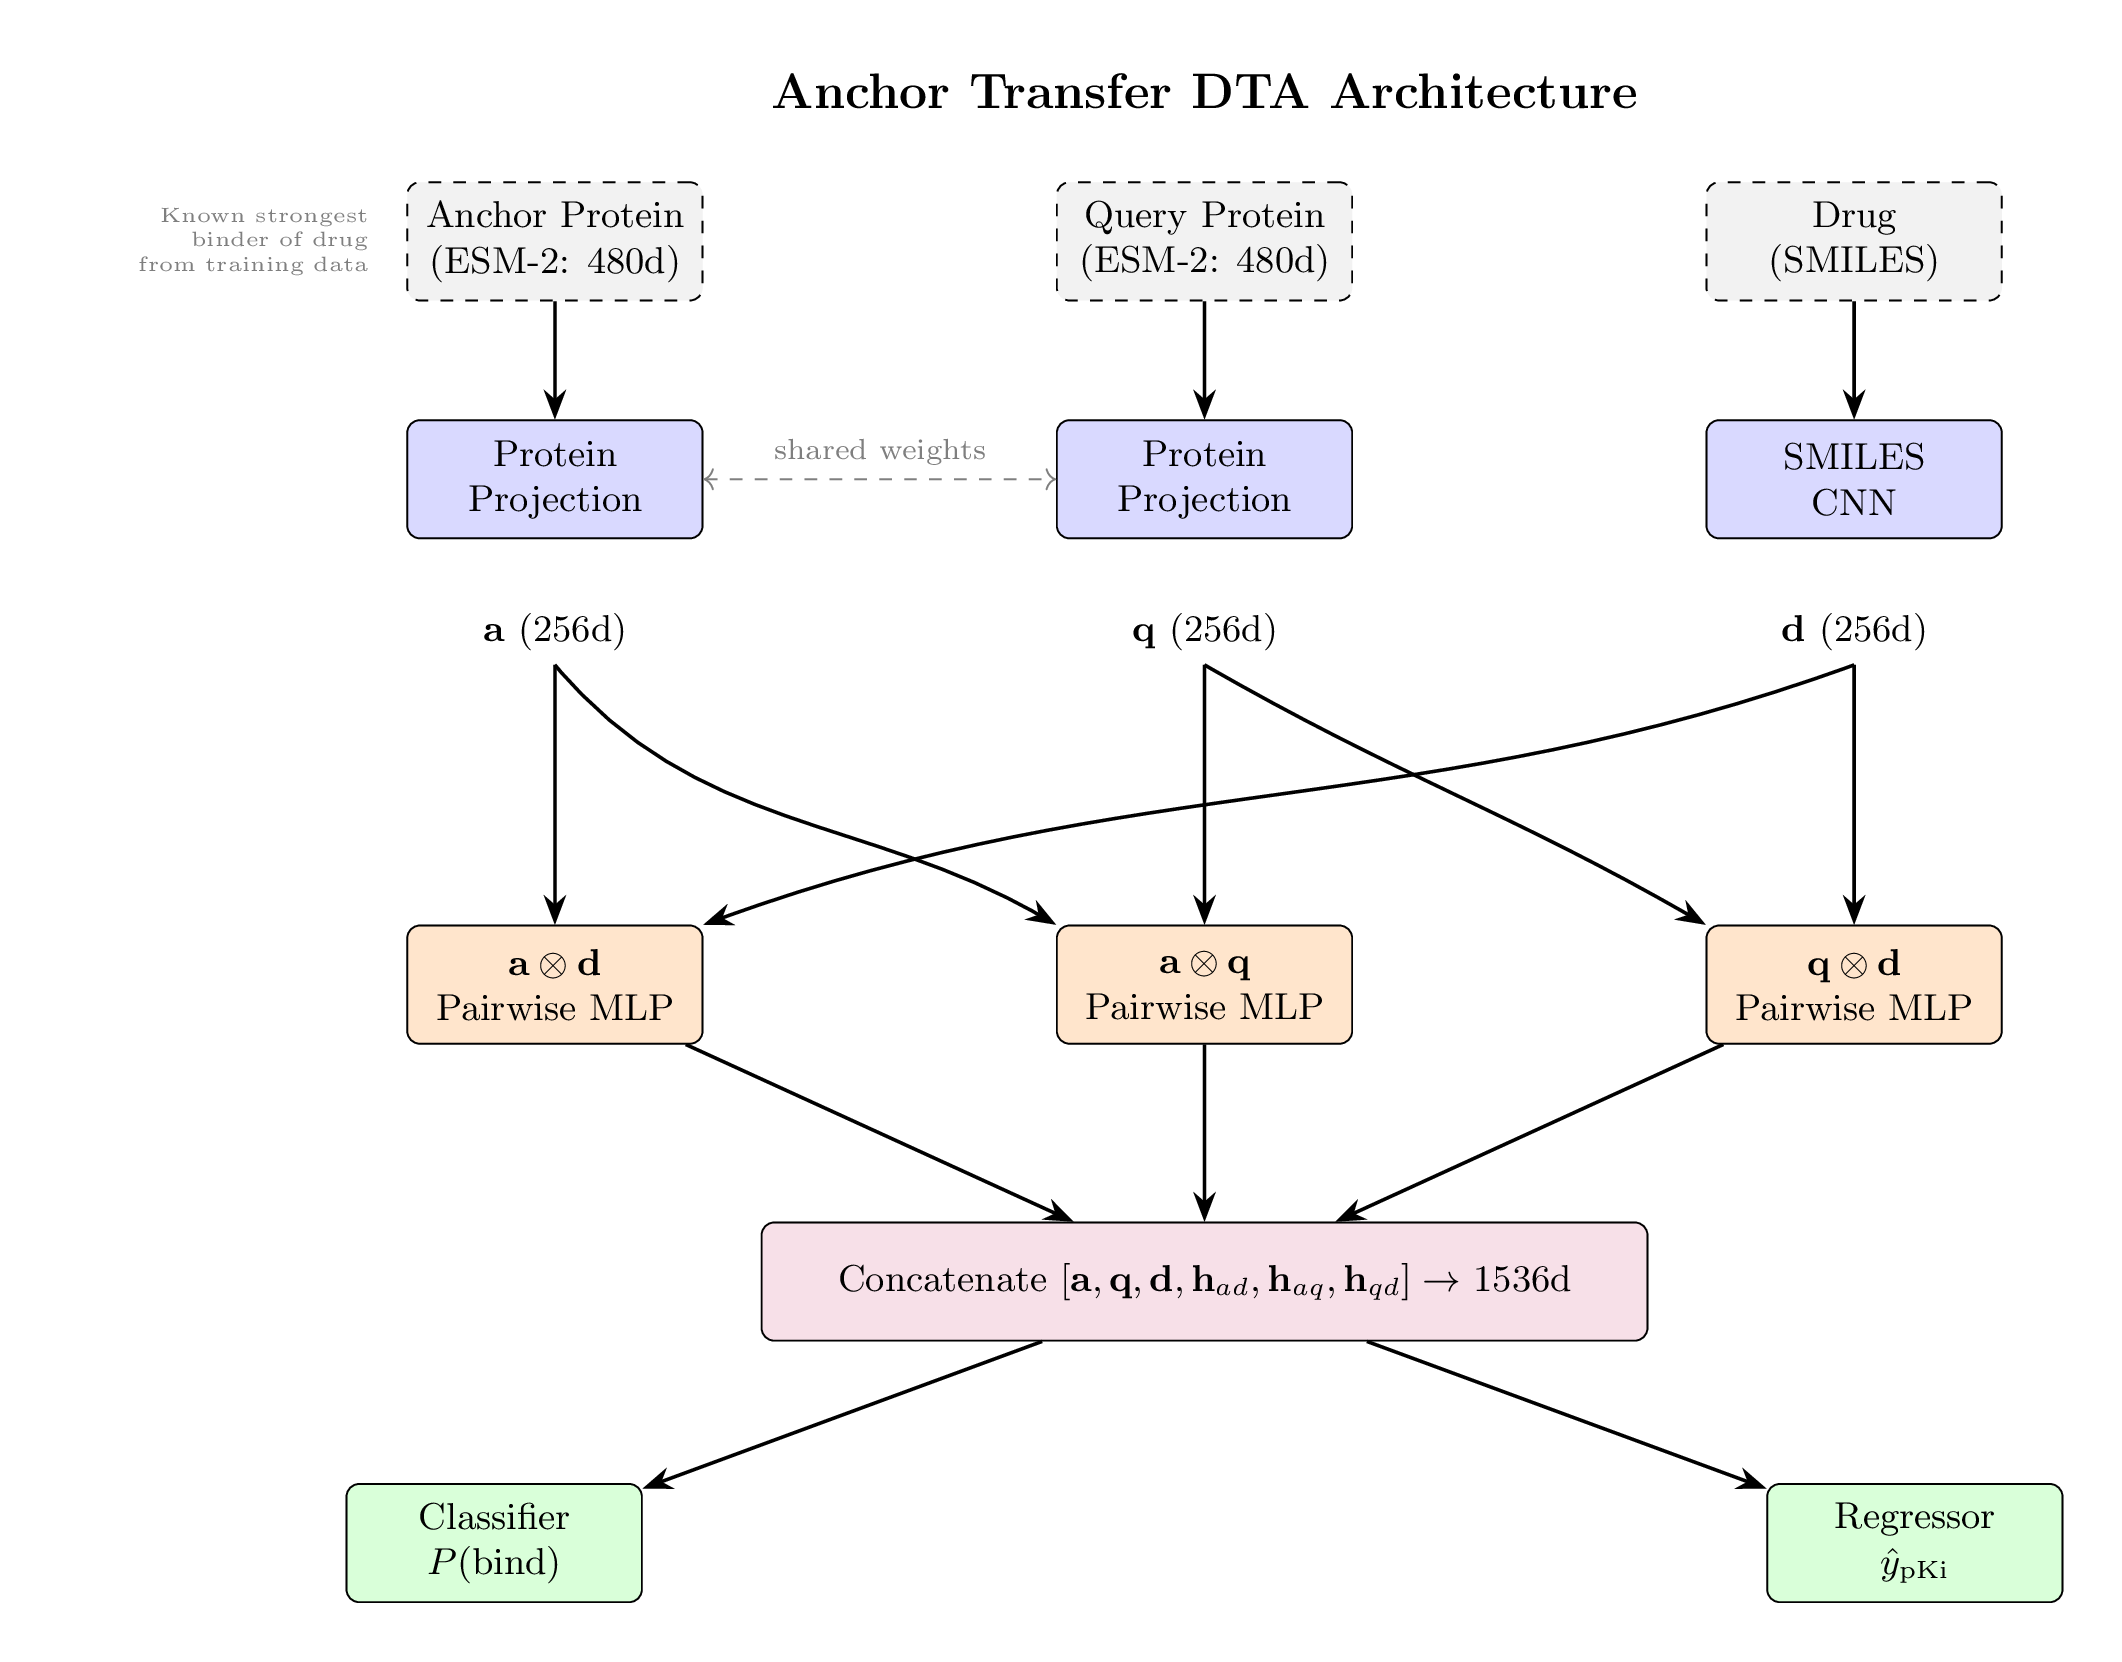
\includegraphics[width=\textwidth]{fig1_architecture.png}
    \caption{Overview of the Anchor Transfer DTA architecture. Given a query protein and a drug, the model retrieves a known strong binder (anchor protein) of that drug. Both proteins are encoded with frozen ESM-2 embeddings projected to a shared 256-dimensional space. The drug is encoded with a parallel SMILES CNN. Three pairwise interaction MLPs model anchor--drug, query--drug, and anchor--query relationships. The fused 1536-dimensional representation feeds dual prediction heads for binding classification and pKi regression.}
    \label{fig:architecture}
\end{figure}

The architecture is deliberately simple. Proteins are encoded with frozen ESM-2 embeddings \cite{lin2023esm2}, drugs with a convolutional encoder over SMILES strings \cite{weininger1988smiles}, and the triplet is processed through three pairwise multilayer perceptrons that model anchor--drug, query--drug, and anchor--query interactions. This keeps the model lightweight while making the transfer pathway explicit.

Because anchor transfer targets generalization rather than benchmark optimization, we evaluate under conditions designed to expose cross-dataset failure. Using DTC as the source, we test on the Davis kinase benchmark \cite{davis2011kinase} (442 kinases, 68 drugs, zero drug overlap with training).

The results confirm that explicit relational transfer is more robust than isolated pair scoring. Crucially, anchors are retrieved at test time from the training set by Tanimoto chemical similarity after excluding canonical chemical duplicates---no oracle access or molecular leakage is involved. On Davis, V2-650M achieves per-protein CI of 0.642 and AUROC of 0.669, while DeepDTA falls to random. Stratifying by anchor binding strength reveals a complementary relationship between encoder capacity and anchor quality: the 650M encoder compensates for weak anchors, while strong anchors equalize the advantage of larger encoders. A cosine similarity ablation shows that 74\% of the model's predictive variance is orthogonal to raw protein similarity, confirming that it learns drug-specific binding patterns beyond nearest-neighbor retrieval.

This paper makes three contributions:
\begin{enumerate}
    \item An \emph{anchor transfer architecture} for DTA that conditions each query on a known strong binder of the same drug, using ESM-2 protein embeddings, a SMILES convolutional encoder, and triple pairwise interaction heads.
    \item A \emph{cross-dataset evaluation protocol} with verified zero drug overlap, anchor-stratified analysis, per-protein metric distributions, and cosine similarity ablation.
    \item \emph{Ablation analyses} showing that anchor quality and encoder capacity are partially substitutable, that structure-aware embeddings (ProstT5) improve transfer, and that the model learns drug-specific patterns beyond raw protein similarity.
\end{enumerate}


\section{Related Work}

Drug-target affinity (DTA) prediction has been dominated by models that score a protein-drug pair directly from sequence or molecular representations. \emph{DeepDTA} established a strong sequence-based baseline by encoding protein sequences and SMILES strings \cite{weininger1988smiles} with convolutional neural networks and learning affinity from the concatenated pair representation \cite{ozturk2018deepdta}. Subsequent work improved the molecular branch while preserving the same pairwise formulation. \emph{GraphDTA} replaced the SMILES convolution with graph neural networks over molecular graphs, arguing that explicit molecular topology yields a stronger drug representation than a character sequence alone \cite{nguyen2021graphdta}. \emph{MolTrans} moved further toward learned cross-modal interaction modelling through a transformer architecture that operates on protein and compound substructures, improving benchmark performance on standard DTA splits \cite{huang2021moltrans}. Other representative models in this family include WideDTA \cite{ozturk2019widedta}, which adds protein motif and domain features, AttentionDTA \cite{zhao2023attentiondta}, which applies attention mechanisms to protein-drug pairs, and MGraphDTA \cite{yang2022mgraphdta}, which introduces multiscale graph encoders for molecular graphs. These models differ in encoder choice, but they share the assumption that the prediction problem is fundamentally pairwise: given $(p,d)$, infer affinity from that pair in isolation.

More recent work has explored alternative interaction modelling paradigms. DrugBAN \cite{bai2023drugban} introduces bilinear attention with domain adaptation to improve cross-domain DTI prediction, sharing our motivation of robustness under distribution shift. SimBoost \cite{he2017simboost} uses gradient boosting with network-based similarity features to capture relational structure between drugs and targets. Tsubaki et al.\ \cite{tsubaki2019compound} combine graph neural networks for compounds with recurrent encoders for proteins using an attention mechanism for end-to-end compound-protein interaction prediction. \emph{ConPlex} is particularly relevant to our setting because it combines a pretrained protein language model with lightweight chemical features \cite{singh2023conplex}. ConPlex constructs a contrastive co-embedding space using ProtBERT \cite{elnaggar2022prottrans} for proteins and Morgan fingerprints \cite{rogers2010morgan} for compounds, and then predicts interaction compatibility from distances in that shared latent space. This design improves efficiency and leverages large-scale protein pretraining, but it still treats affinity prediction as matching between independently encoded proteins and drugs rather than transfer from a known binding reference.

A complementary line of work uses three-dimensional structure. Structure-based docking methods can in principle model geometric complementarity more directly than sequence-only DTA models \cite{kitchen2004docking}, but they usually require reliable ligand poses or receptor conformations. DiffDock \cite{corso2023diffdock} is representative of this direction: it uses a diffusion process to generate docking poses and has shown strong performance for pose prediction, yet it depends on explicit 3D inputs for both ligand and protein and is therefore limited by structure availability and conformational uncertainty. The rapid expansion of predicted structures through AlphaFold \cite{jumper2021alphafold} and RoseTTAFold \cite{baek2021rosettafold} has made structure-aware screening more practical even for proteins lacking experimental complexes. Related protein language model systems such as ESMFold further reduce the cost of producing approximate structural models at scale \cite{lin2023esm2}. Even so, AlphaFold-based DTA pipelines typically remain structure-conditioned pairwise predictors; they address missing structure, but not the problem of transferring interaction evidence across datasets.

Protein language models have also become central to modern DTA. Large pretrained sequence encoders, including ESM-1b \cite{rives2021biological}, ProtTrans \cite{elnaggar2022prottrans} and the TAPE benchmarking framework \cite{rao2019evaluating}, have demonstrated that self-supervised pretraining on evolutionary sequences can provide richer protein features than character-level embeddings. ESM-2 in particular has emerged as a strong general-purpose protein representation model \cite{lin2023esm2}. In DTA, these embeddings are often used as frozen protein features that are combined with a drug encoder and passed to a regression or classification head \cite{li2022effective}. Our ESM-DTA baseline follows this pattern by replacing DeepDTA's learned protein embedding branch with frozen ESM-2 features while keeping the drug-side convolutional encoder. This comparison is important because it separates the value of a stronger protein representation from the value of changing the prediction formulation itself.

The evaluation practices in the DTA literature also deserve attention. Most published models are evaluated on random splits of standard benchmarks such as Davis \cite{davis2011kinase} or DTC \cite{tang2014dtc}, where significant overlap between training and test sets can inflate performance estimates. Pahikkala et al.\ \cite{pahikkala2015kronrls} showed that evaluation under cold-start (unseen protein or drug) settings is much harder, and Mayr et al.\ \cite{mayr2018deeptox} demonstrated large performance gaps across different assay collections. More recently, low-data and few-shot approaches for drug discovery have been explored \cite{altae2017low}, but these focus on learning from limited labelled examples rather than on transferring binding evidence from known interactions in a different dataset.

Taken together, prior work has substantially improved in-distribution DTA accuracy through better sequence encoders, graph encoders, transformers, contrastive co-embeddings and structure-aware docking. However, the dominant evaluation paradigm still emphasizes performance within a benchmark or on random splits of a single resource. To our knowledge, no prior DTA method explicitly frames \emph{cross-dataset transfer} as the core problem by conditioning each query on a known strong binder of the same drug. This gap motivates the present work: rather than only improving how a single protein-drug pair is encoded, we ask whether known interaction evidence can be reused as an anchor to improve generalization across datasets, protein families and difficult regimes such as intrinsically disordered proteins.


\section{Methods}

\subsection{Problem formulation}

We study drug-target affinity prediction under an anchor-transfer formulation. Instead of scoring a protein-drug pair in isolation, the model receives an anchor protein $a$, a query protein $q$, and a drug $d$, and predicts both a continuous affinity value and a binary binding score:
\[
f(a,q,d)\rightarrow (\hat{y},\hat{b}),
\]
where $\hat{y}$ is the predicted pKi and $\hat{b}\in[0,1]$ is the predicted binding probability. The central idea is that the anchor provides binding-specific context for the query drug. If a drug is already known to bind one protein strongly, the model can ask whether the query protein is compatible with that same binding context. This formulation draws on the broader principle of transfer learning \cite{pan2010transfer}, in which knowledge from a source domain (the known anchor interaction) is reused to improve prediction in a target domain (the unseen query interaction).

For each drug in the training set, we define the anchor as the protein with the highest observed pKi for that drug. Thus, given a query pair $(q,d)$, the corresponding anchor $a(d)$ is the strongest known binder of $d$ in the source data. When the query protein itself is the top-ranked binder, we use the next-highest protein so that the anchor and query are not identical. This produces training triplets of the form $(a,q,d)$ with supervision on the affinity of the query pair $(q,d)$.

We train the model jointly for regression and classification, following a multitask learning approach \cite{caruana1997multitask}. Continuous affinity supervision uses the observed pKi value $y$, while the binary target is derived by thresholding pKi into confident binders and non-binders. We assign $b=1$ when $y\geq 7$, $b=0$ when $y\leq 5$, and treat the intermediate range $5<y<7$ as ambiguous. These samples remain useful for regression but are excluded from the binary loss. This multitask setup lets the model learn both fine-grained affinity ranking and coarse binding discrimination.

\subsection{Anchor transfer architecture}

Figure~\ref{fig:architecture} summarizes the proposed model. The architecture contains a shared protein encoder, a shared drug encoder, three pairwise interaction multilayer perceptrons, and two prediction heads. The shared encoders produce aligned 256-dimensional embeddings for the anchor protein, query protein and drug; the interaction blocks then model all pairwise relations inside the triplet.

\subsection{Protein encoder}

Each protein is represented by a frozen embedding from ESM-2 \cite{lin2023esm2}. We use either the 35M model, which produces a 480-dimensional sequence embedding, or the 650M model, which produces a 1,280-dimensional embedding. The pretrained ESM-2 parameters are kept fixed throughout training, consistent with the common practice of using frozen protein language model features for downstream prediction tasks \cite{rives2021biological,rao2019evaluating}. To map both anchor and query proteins into the same task-specific space, we apply the same projection module to both branches:
\[
h_p = \mathrm{LayerNorm}\!\left(\mathrm{ReLU}(W_p x_p + b_p)\right),
\]
where $x_p\in\mathbb{R}^{480}$ or $\mathbb{R}^{1280}$ is the frozen ESM-2 representation, $h_p\in\mathbb{R}^{256}$ is the projected embedding, and LayerNorm denotes layer normalization \cite{ba2016layernorm}. Weight sharing is important here: anchor and query proteins must be directly comparable, so they are encoded with the same linear projection, nonlinearity and normalization pipeline.

\subsection{Drug encoder}

Drugs are encoded from SMILES strings \cite{weininger1988smiles} using a compact convolutional encoder inspired by DeepDTA \cite{ozturk2018deepdta}. After token embedding, the SMILES sequence is processed by three parallel one-dimensional convolution branches with kernel sizes 4, 6 and 8. Each branch uses 32 filters followed by global max pooling. The pooled branch outputs are concatenated into a 96-dimensional drug feature,
\[
z_d = \big[\mathrm{pool}(\mathrm{Conv}_4(d)) \,\|\, \mathrm{pool}(\mathrm{Conv}_6(d)) \,\|\, \mathrm{pool}(\mathrm{Conv}_8(d))\big]\in\mathbb{R}^{96},
\]
and a final linear projection maps this vector to the shared 256-dimensional latent space:
\[
h_d = W_d z_d + b_d.
\]
Using parallel kernels allows the encoder to capture SMILES motifs of different lengths while keeping the drug branch lightweight.

\subsection{Triple pairwise interaction module}

Once the three entities are encoded, the model explicitly constructs interaction features for every pair in the triplet. Let $h_a$, $h_q$ and $h_d$ denote the 256-dimensional embeddings of the anchor protein, query protein and drug. We then compute
\[
h_{ad} = \phi_{ad}([h_a \| h_d]), \qquad
h_{qd} = \phi_{qd}([h_q \| h_d]), \qquad
h_{aq} = \phi_{aq}([h_a \| h_q]),
\]
where each $\phi$ is an independent pairwise multilayer perceptron that takes the 512-dimensional concatenated input and projects it to 256 dimensions followed by a ReLU nonlinearity. These three learned features capture distinct aspects of the problem: the anchor-drug branch represents evidence that the drug already binds a known reference protein, the query-drug branch represents direct compatibility between the query and the compound, and the anchor-query branch represents similarity or complementarity between the reference protein and the query.

\subsection{Fusion and prediction heads}

The final representation concatenates the three base embeddings and the three pairwise features:
\[
z = [h_a \| h_q \| h_d \| h_{ad} \| h_{qd} \| h_{aq}] \in \mathbb{R}^{1536}.
\]
This fused vector is passed to two task-specific heads. The classifier predicts binding probability through a multilayer perceptron followed by a sigmoid output, while the regressor predicts continuous pKi with the same hidden structure but a linear output. The classifier is optimized for binary binding discrimination, whereas the regressor preserves the quantitative affinity signal. In practice, the dual-head design is useful because AUROC and pKi regression quality do not always move together under dataset shift.

\subsection{Training objective}

The overall loss combines binary cross-entropy and mean squared error:
\[
\mathcal{L} = \mathcal{L}_{\mathrm{BCE}} + \alpha \mathcal{L}_{\mathrm{MSE}}.
\]
In all experiments, we set $\alpha=1.0$.
The regression loss is computed over all examples,
\[
\mathcal{L}_{\mathrm{MSE}} = \frac{1}{N}\sum_{i=1}^{N}(\hat{y}_i-y_i)^2,
\]
whereas the classification loss is masked so that ambiguous affinities do not contribute. Defining
\[
m_i=
\begin{cases}
1, & y_i\leq 5 \text{ or } y_i\geq 7, \\
0, & 5<y_i<7,
\end{cases}
\]
we compute
\[
\mathcal{L}_{\mathrm{BCE}} =
\frac{1}{\sum_i m_i}
\sum_{i=1}^{N}
m_i\,\mathrm{BCE}(\hat{b}_i,b_i).
\]
This masking scheme preserves the full pKi range for regression while avoiding noisy supervision near the decision boundary. It also matches the evaluation setting, where binary discrimination is most meaningful for clearly binding and clearly non-binding interactions.

\subsection{Drug-anchor ablation}

To test whether the gains come from protein-side anchoring specifically or from conditioning on any known same-partner example, we evaluate a drug-anchor ablation. In this variant, the inputs are an anchor drug $a_d$, a query drug $q_d$, and a protein $p$, and the model predicts pKi for the query pair:
\[
f(a_d,q_d,p)\rightarrow \hat{y}.
\]
The protein branch remains the frozen ESM-2 projection, while the anchor-drug and query-drug branches share the same SMILES convolutional encoder. Pairwise interaction blocks are built for $(a_d,p)$, $(q_d,p)$ and $(a_d,q_d)$, mirroring the structure of the main model. This ablation tests whether transferable context is still useful when the anchor is moved to the compound side rather than the protein side.

\subsection{ESM-DTA baseline}

As a pairwise baseline, we construct \emph{ESM-DTA} by replacing DeepDTA's learned protein character embedding pathway with frozen ESM-2 features \cite{lin2023esm2}. The drug encoder remains the same DeepDTA-style SMILES convolution used in the main model, but the input is only the pair $(q,d)$ and there is no anchor. Protein and drug embeddings are concatenated and passed to a standard multilayer perceptron to predict affinity. This baseline is intentionally simple: it asks whether stronger pretrained protein representations alone are sufficient, or whether the improvement instead comes from explicitly conditioning prediction on a known strong binder for the same drug.

\subsection{Conformation weighting analysis}

As an auxiliary analysis for IDP queries, we replaced the query protein's ESM-2 embedding with a TM-weighted average of ESM-2 embeddings from structurally matched ordered proteins. The matches were obtained by running Foldseek on IDRome conformations and aggregating the retrieved ordered-protein embeddings by TM-score, while leaving the rest of the model and evaluation protocol unchanged.


\section{Experimental Setup}

\subsection{Training Datasets}

We trained the main models on Drug Target Commons (DTC) only \cite{tang2014dtc}, comprising 401,978 drug-target interactions spanning 2,827 proteins and 164,831 drugs. We retained pKi values derived from Ki measurements in order to keep the supervision signal on a consistent inhibition-constant scale. Proteins were split at the entity level into 80\% training, 10\% validation and 10\% test partitions with random seed 42, ensuring that proteins in the evaluation partitions were not observed during training.

BindingDB \cite{gilson2016bindingdb} was used only as a robustness check rather than as a second training source. In particular, a BindingDB-trained V2 model reached AUROC 0.665 on Davis, versus 0.714 for the matched DTC-trained V2 model, indicating that the main conclusions do not depend on dual-dataset training.

\subsection{External Evaluation Benchmarks}

External evaluation was designed to stress cross-dataset generalization rather than within-dataset interpolation. For all external benchmarks, overlap with DTC was explicitly checked at the protein, drug and interaction levels where applicable, and datasets with excessive overlap were excluded from analysis.

The Davis kinase benchmark \cite{davis2011kinase} contains 30,056 kinase-drug interactions over 442 proteins and 68 drugs. Davis reports dissociation constants (Kd) rather than inhibition constants (Ki). We treat pKd and pKi interchangeably for ranking evaluation, as both measure binding strength on comparable logarithmic scales. This is a common simplification in DTA benchmarks. Davis provides a strict compound novelty test relative to DTC, with 0\% drug overlap, and is highly imbalanced after thresholding because approximately 70\% of values are censored at pKi$=5$.

We additionally analyze the Metz kinase benchmark, which spans 35,259 interactions over 170 proteins and 1,423 drugs. Unlike Davis, Metz exhibits extensive overlap with the DTC training reference at both the protein and chemical levels. For the benchmark visualization analyses in Section~\ref{sec:benchmark_heatmaps}, we therefore report \emph{two} protocols side by side: an \emph{unfiltered} view that retains all anchorable benchmark interactions after model-coverage checks, and a \emph{filtered} view that removes proteins overlapping the DTC training set by entity or exact sequence and removes drugs overlapping the DTC training set by canonical SMILES or full InChIKey before anchors are defined. Under this stricter filtered protocol, Davis contracts from 30,056 interactions over 442 proteins and 68 drugs to 854 interactions over 122 proteins and 7 drugs, while Metz contracts from 35,259 interactions over 170 proteins and 1,423 drugs to 374 interactions over 9 proteins and 115 drugs.

\subsection{Overlap Verification and Baselines}

Table~\ref{tab:overlap_verification} summarizes the verified overlap statistics for the external dataset. Davis satisfies zero drug overlap with DTC. Notably, 77\% of Davis proteins share sequences with DTC training proteins, meaning the evaluation primarily tests compound novelty (new drugs for known protein families) rather than dual novelty.

We compared Anchor Transfer Learning against three representative baselines. DeepDTA \cite{ozturk2018deepdta} serves as a strong sequence-and-SMILES convolutional baseline for pairwise affinity prediction. We report a modified re-implementation of ConPlex as ConPlex*, using ESM-2 embeddings and a SMILES CNN encoder instead of the original ProtBERT and Morgan fingerprints, to isolate the effect of the contrastive training objective from encoder choice. We also evaluated ESM-DTA as a second ESM-based baseline to test whether gains arise from stronger protein representations alone or from the anchor-transfer formulation itself. We refer to the anchor transfer model with ESM-2 35M as V2-35M, with ESM-2 650M as V2-650M, the drug-side anchor variant as Drug-Anchor, and the ESM-2 baseline without anchors as ESM-DTA.

\begin{table}[t]
\centering
\caption{Overlap between DTC training set and the Davis benchmark. Raw SMILES comparison (commonly used in DTA literature) reports 0\% drug overlap, but canonical chemical identity reveals 83.8\% overlap. All canonical duplicates are excluded from the anchor retrieval pool before evaluation.}
\label{tab:overlap_verification}
\begin{tabular}{lcc}
\toprule
Overlap level & Davis--DTC & Note \\
\midrule
Protein (by sequence) & 77\% & Same kinases, different drugs \\
Drug (raw SMILES) & 0\% & String identity only \\
Drug (canonical SMILES) & 83.8\% & True molecular identity \\
Drug (InChIKey) & 89.7\% & Gold-standard identity \\
\bottomrule
\end{tabular}
\end{table}

\subsection{Evaluation Protocol and Hyperparameters}

External benchmarks were evaluated with anchors retrieved from the DTC training set by Tanimoto chemical similarity (chirality-aware Morgan fingerprints, radius 2, 2048 bits). All canonical chemical duplicates of evaluation drugs are explicitly excluded from the retrieval pool before searching, ensuring genuine zero molecular overlap between retrieved anchors' drugs and evaluation compounds. For each query drug, we select the most similar remaining DTC drug whose strongest binder has pKi~$\geq 7$ as the anchor protein. We report AUROC, concordance index (CI) \cite{gonen2005concordance}, average precision (AUPRC), and root mean squared error (RMSE).

For the benchmark heatmaps and quartile-wise distribution plots, we compare the unfiltered and filtered protocols directly. The unfiltered protocol retains all anchorable benchmark interactions after requiring model coverage (protein sequences plus ESM embeddings where needed). The filtered protocol additionally removes benchmark proteins overlapping the DTC training set at the entity or exact-sequence level and benchmark drugs overlapping the DTC training set at the canonical-SMILES or full-InChIKey level. These figures report \emph{per-protein} CI summaries rather than pooled interaction-level metrics. We restrict the visual comparison to V2 oracle/weakest/random controls, DeepDTA, ConPlex*, and ESM-DTA. DrugBAN is omitted from the main-paper comparison because its graph-based drug encoder changes the input modality and would conflate the anchor-transfer question with a separate molecular representation change.

Unless otherwise stated, all models were trained with batch size 512 using AdamW \cite{loshchilov2019adamw} with learning rate $10^{-3}$. We applied cosine annealing learning-rate decay, early stopping with patience 20 based on validation performance, and gradient clipping with maximum norm 1.0. These hyperparameters were held fixed across experiments to isolate the effect of the modeling choice rather than benchmark-specific tuning.

\subsection{Code Availability}

Code, benchmark preprocessing, overlap-audit utilities, and figure-generation scripts are available at \url{https://github.com/Basartemiz/IDR-GAT}. The repository includes the training and evaluation entry points used for the main DTC, Davis, and Metz analyses.


\section{Results}

We evaluated the proposed model family on a common anchored subset of the DTC test split and on external benchmarks designed to stress transfer beyond the source dataset. The overall pattern is consistent across settings: architectures that are strongest on same-dataset evaluation are not necessarily the ones that generalize best. Figure~\ref{fig:cross_dataset} summarizes this ranking shift across benchmarks, and Figure~\ref{fig:gen_gap} makes the same point more directly by plotting same-dataset performance against Davis transfer. The resulting generalization gap is the main empirical phenomenon of the paper.

\begin{figure}[t]
    \centering
    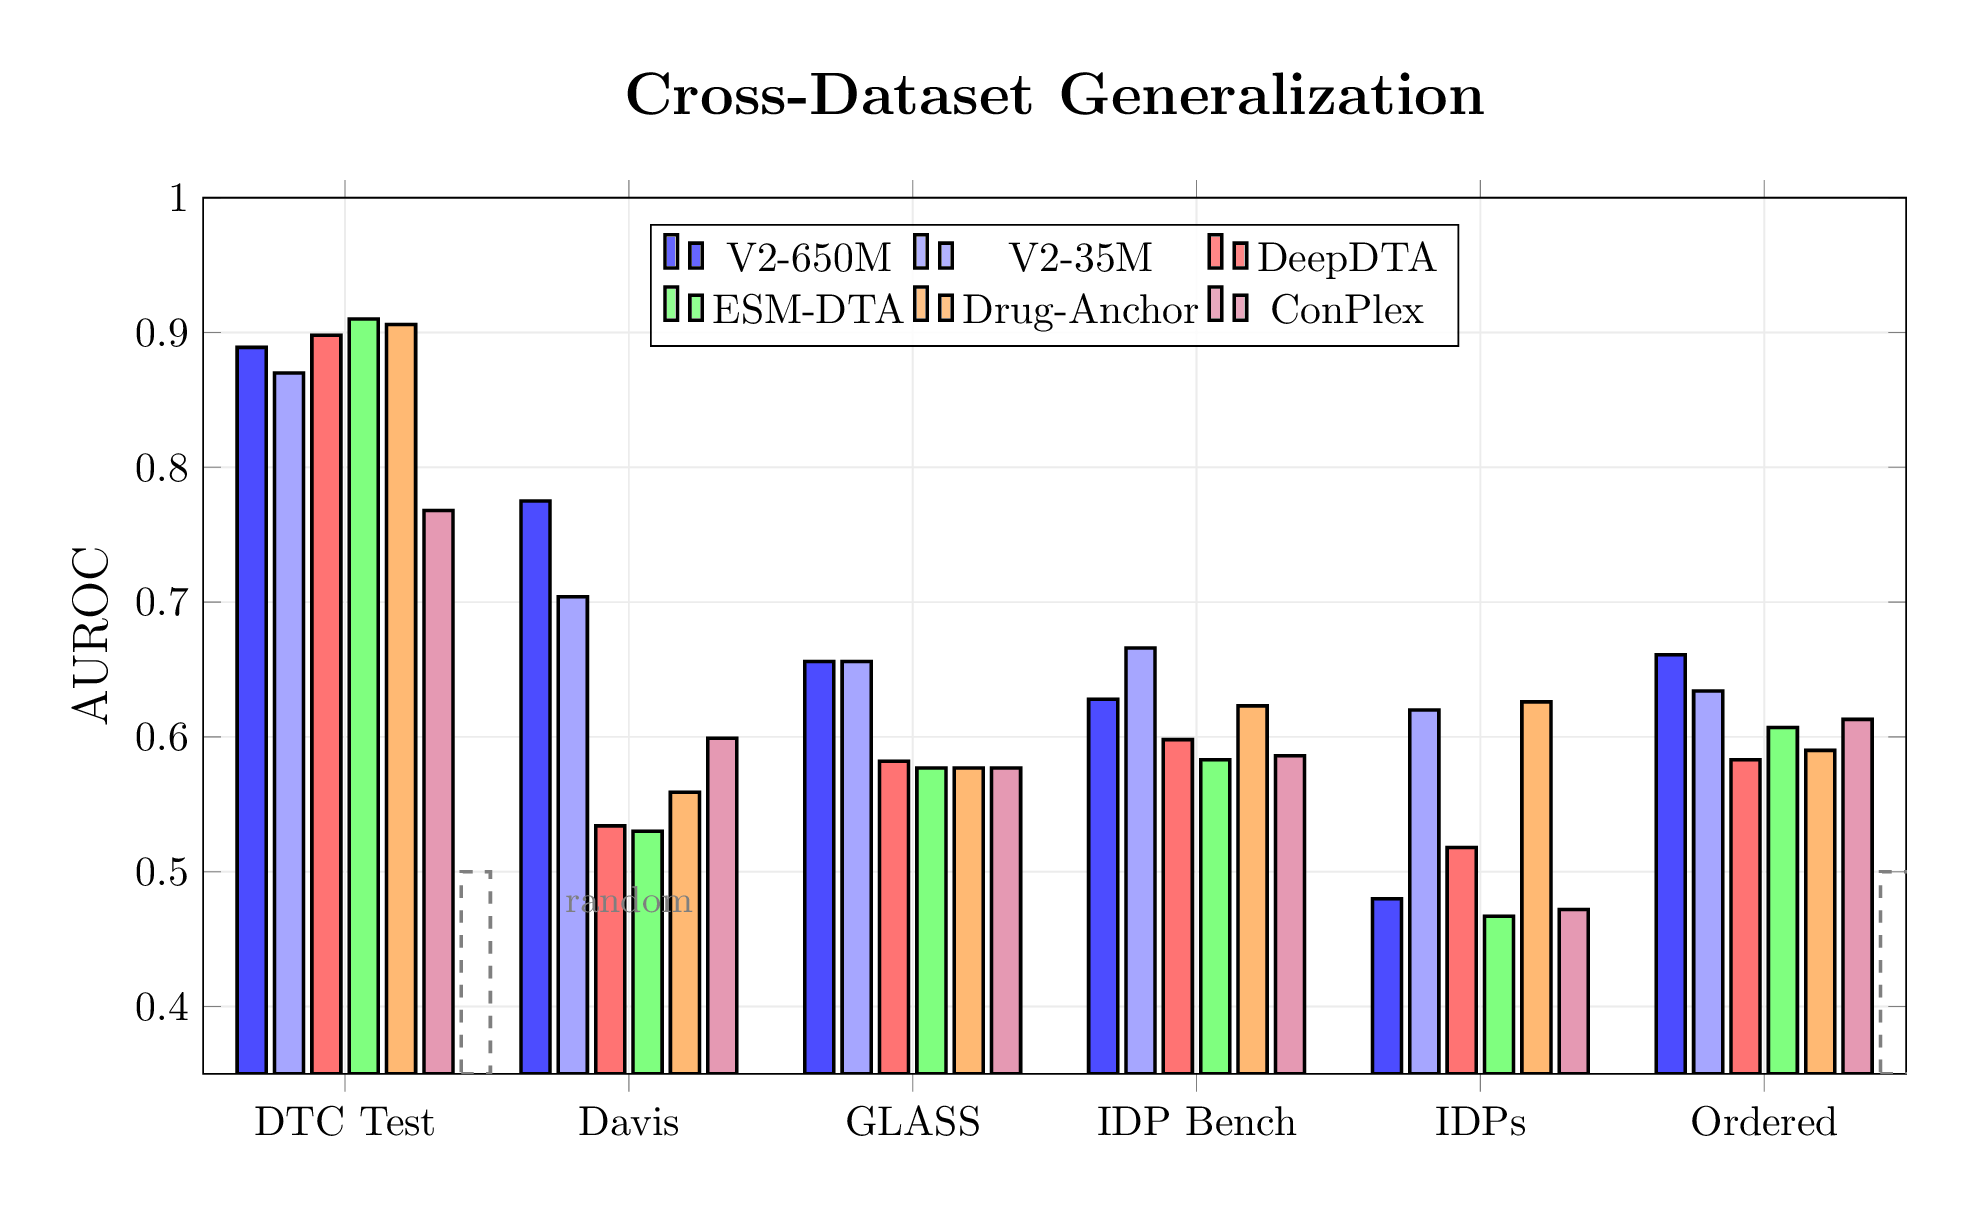
\includegraphics[width=\textwidth]{fig2_cross_dataset.png}
    \caption{Cross-dataset generalization across all benchmarks. All models are trained on DTC and evaluated on the same anchored interaction subsets. Anchor transfer variants (V2-650M, V2-35M) maintain strong performance under distribution shift, while pairwise baselines (DeepDTA, ESM-DTA) that excel on DTC collapse on external benchmarks.}
    \label{fig:cross_dataset}
\end{figure}

\begin{figure}[t]
    \centering
    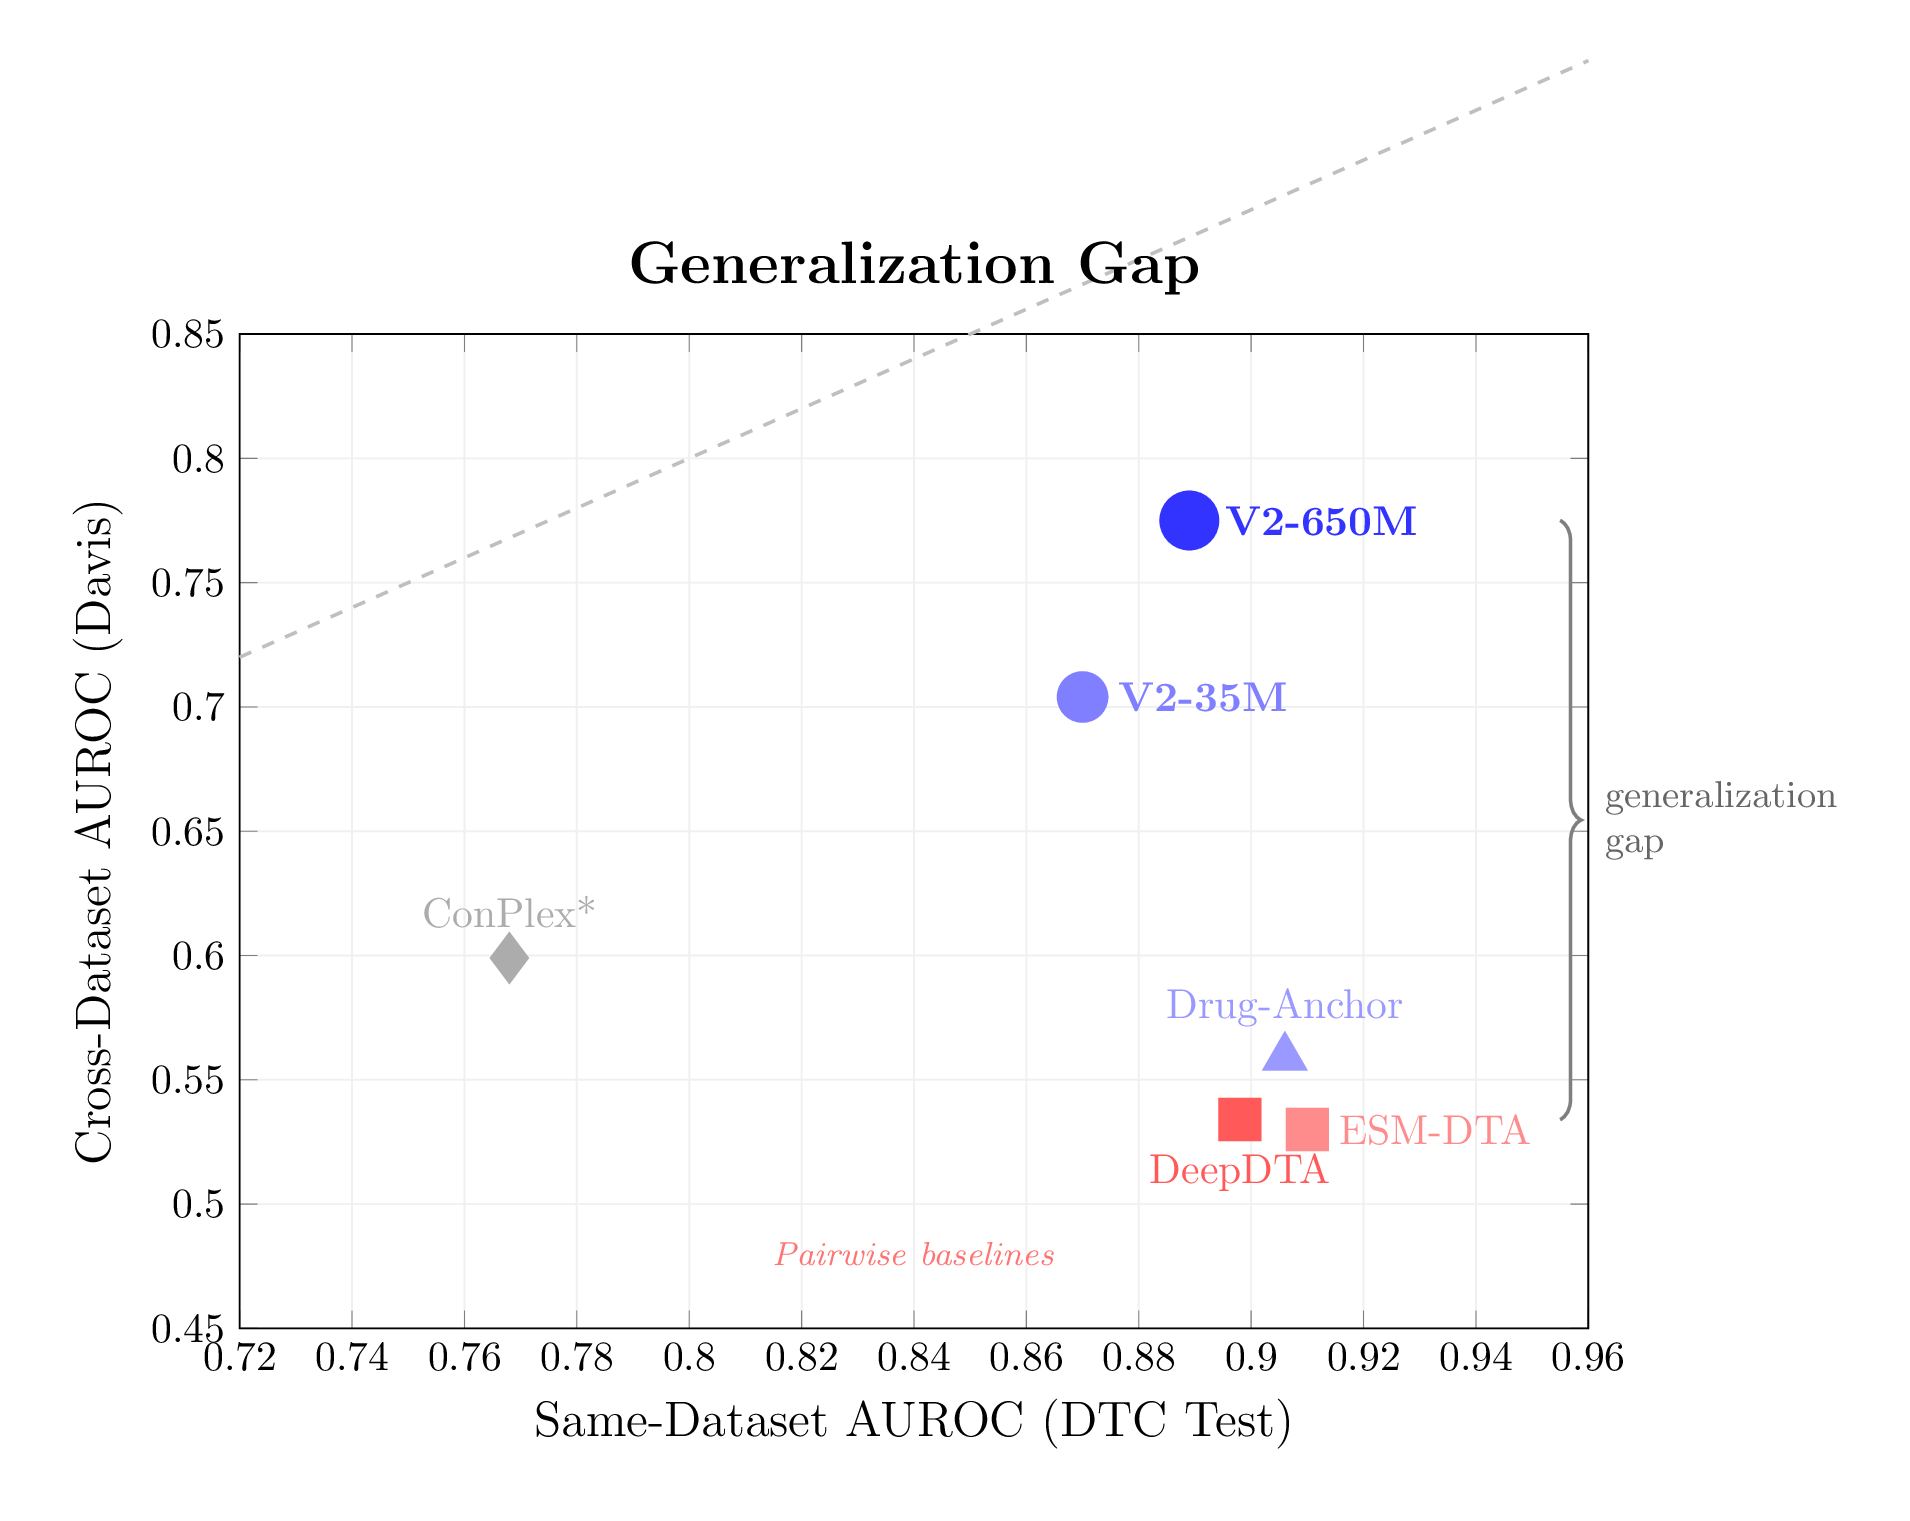
\includegraphics[width=0.7\textwidth]{fig3_generalization_gap.png}
    \caption{Generalization gap: same-dataset AUROC (DTC test) versus cross-dataset AUROC (Davis). The dashed diagonal represents perfect generalization. Anchor transfer models (blue markers) cluster near the diagonal, while pairwise baselines (red squares) show large drops, indicating memorization of dataset-specific patterns rather than learning transferable binding features.}
    \label{fig:gen_gap}
\end{figure}

\subsection{Same-Dataset}

Table~\ref{tab:dtc_test} reports performance on the common DTC test subset ($n=27{,}536$). All sequence-based models are strong in this regime, with AUROC values between 0.870 and 0.910 (Figure~\ref{fig:same_dataset}). ESM-DTA is the best same-dataset model, reaching AUROC 0.910 together with the best CI and RMSE. Drug-Anchor and DeepDTA follow closely, while the two V2 variants lag slightly despite using the same frozen ESM-2 representation family.

\begin{figure}[t]
    \centering
    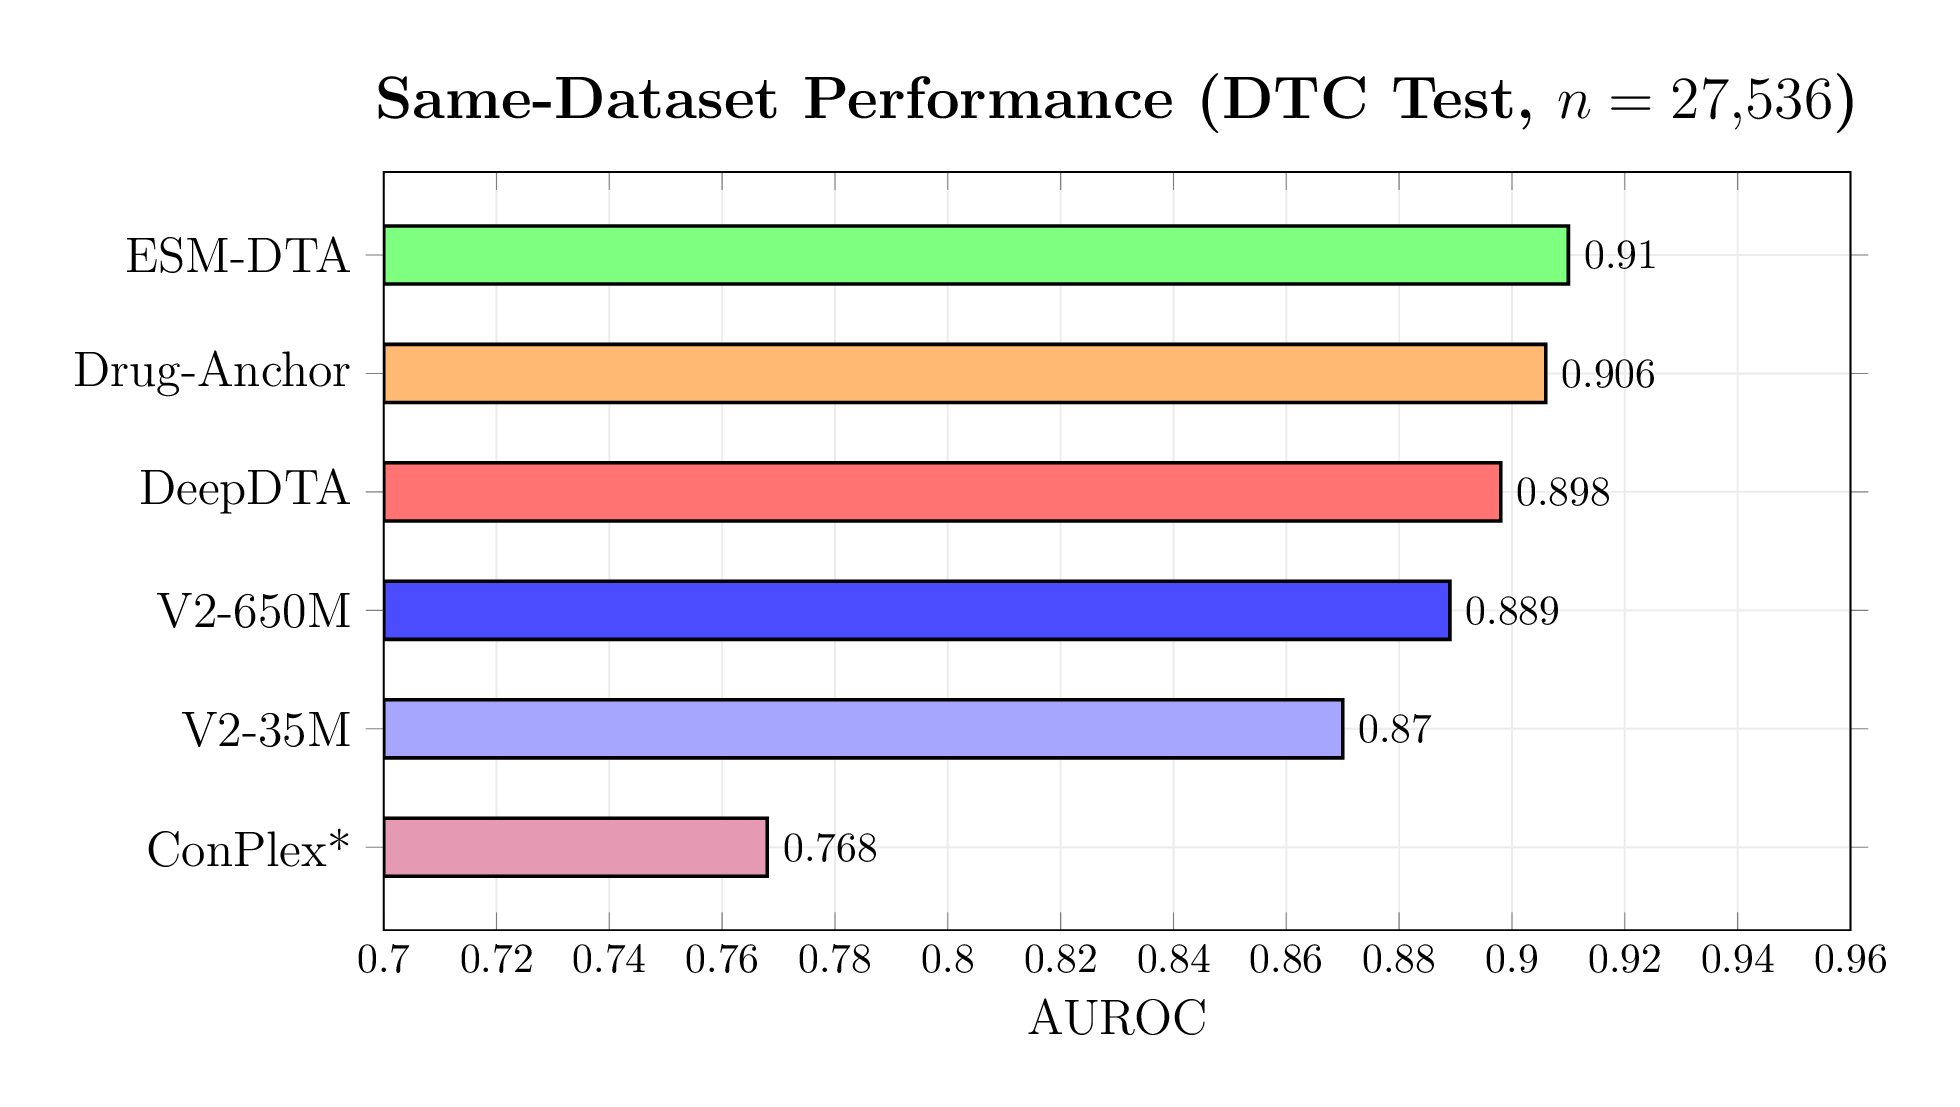
\includegraphics[width=0.85\textwidth]{fig5_same_dataset.png}
    \caption{Same-dataset AUROC on the DTC test set ($n=27{,}536$). All models perform well in-distribution, with ESM-DTA and Drug-Anchor leading. This ranking reverses under cross-dataset evaluation (cf.\ Figure~\ref{fig:cross_dataset}).}
    \label{fig:same_dataset}
\end{figure}

This same-dataset ranking is important because it establishes that stronger within-benchmark performance is not the same as stronger transfer. The best source-distribution model later becomes one of the weakest external models. Figure~\ref{fig:gen_gap} visualizes this reversal by contrasting DTC AUROC with Davis AUROC across methods.

\begin{table}[t]
\centering
\caption{Same-dataset performance on the common anchored DTC test set ($n=27{,}536$). Dashes indicate metrics unavailable for ConPlex*.}
\label{tab:dtc_test}
\small
\begin{tabular}{lccc}
\toprule
Model & AUROC & CI & RMSE \\
\midrule
ESM-DTA & \textbf{0.910} & \textbf{0.791} & \textbf{0.738} \\
Drug-Anchor & 0.906 & 0.786 & 0.783 \\
DeepDTA & 0.898 & 0.775 & 0.776 \\
V2-650M & 0.889 & 0.775 & 0.816 \\
V2-35M & 0.870 & 0.747 & 0.901 \\
ConPlex* & 0.768 & 0.680 & -- \\
\bottomrule
\end{tabular}
\end{table}

\subsection{Cross-Dataset Generalization}
\label{sec:cross_dataset}

The Davis benchmark produces the clearest cross-dataset ranking reversal. At test time, anchors are retrieved from the DTC training set by Tanimoto chemical similarity (chirality-aware Morgan fingerprints, radius 2, 2048 bits) after explicitly excluding all canonical chemical duplicates of Davis drugs from the retrieval pool. This ensures strict zero molecular overlap between training anchors and evaluation compounds. We verified overlap at six levels (Table~\ref{tab:overlap_audit}): while raw SMILES string overlap is 0\%, canonical SMILES overlap is 83.8\% and InChIKey overlap is 89.7\%, confirming that most Davis kinase inhibitors are present in DTC under different string representations. All such duplicates are removed before anchor retrieval.

\begin{table}[t]
\centering
\caption{Drug overlap audit between Davis and the DTC training set at six levels of chemical identity. Raw SMILES string comparison substantially underestimates true overlap.}
\label{tab:overlap_audit}
\small
\begin{tabular}{lcc}
\toprule
Identity level & Overlap & \% \\
\midrule
Raw SMILES string & 0/68 & 0.0 \\
Canonical SMILES & 57/68 & 83.8 \\
Full InChIKey & 61/68 & 89.7 \\
First-block InChIKey (no stereo) & 63/68 & 92.6 \\
Morgan FP (no chirality) & 59/68 & 86.8 \\
Morgan FP (with chirality) & 57/68 & 83.8 \\
\bottomrule
\end{tabular}
\end{table}

After duplicate exclusion, the retrieval achieves 99.7\% coverage ($n=29{,}975$). Table~\ref{tab:davis_cross_dataset} reports results with AUPRC to account for the severe class imbalance (8.6\% binders). V2-650M leads with CI 0.642, AUROC 0.669, and AUPRC 0.209. The absolute drops from Table~\ref{tab:dtc_test} are substantial for pairwise models: DeepDTA and ESM-DTA collapse to near-random. Figure~\ref{fig:gen_gap} highlights this as a generalization-gap effect.

Table~\ref{tab:tanimoto_strat} stratifies V2-650M performance by Tanimoto similarity between the query drug and the retrieved anchor's drug, directly testing how the model performs when the anchor's chemistry differs from the query.

\begin{table}[t]
\centering
\caption{Cross-dataset generalization from DTC to Davis ($n=29{,}975$) after excluding canonical chemical duplicates. Anchors retrieved by Tanimoto similarity from the DTC training set. Per-protein metrics.}
\label{tab:davis_cross_dataset}
\small
\begin{tabular}{lcccc}
\toprule
Model & CI $\uparrow$ & AUROC $\uparrow$ & AUPRC $\uparrow$ & RMSE $\downarrow$ \\
\midrule
V2-650M & \textbf{0.642} {\scriptsize [.634--.651]} & \textbf{0.669} {\scriptsize [.653--.686]} & \textbf{0.209} {\scriptsize [.192--.227]} & \textbf{0.923} \\
V2-35M  & 0.591 {\scriptsize [.583--.599]} & 0.618 {\scriptsize [.603--.634]} & 0.171 {\scriptsize [.157--.186]} & 1.069 \\
DeepDTA & 0.521 {\scriptsize [.513--.528]} & 0.504 {\scriptsize [.487--.521]} & 0.155 {\scriptsize [.141--.170]} & 1.157 \\
ESM-DTA & 0.501 {\scriptsize [.495--.507]} & 0.503 {\scriptsize [.488--.519]} & 0.140 {\scriptsize [.129--.152]} & 1.299 \\
\bottomrule
\end{tabular}
\end{table}

\begin{table}[t]
\centering
\caption{V2-650M performance stratified by Tanimoto similarity between the query drug and the retrieved anchor's drug. After excluding canonical duplicates, no exact matches remain. The model generalizes even to chemically dissimilar compounds (Tanimoto~$< 0.6$), with the best performance at moderate similarity (0.6--0.8).}
\label{tab:tanimoto_strat}
\small
\begin{tabular}{lccccc}
\toprule
Tanimoto bin & $n$ & Drugs & CI $\uparrow$ & AUROC $\uparrow$ & AUPRC $\uparrow$ \\
\midrule
{[0--0.6)}   & 14,992 & 34 & 0.656 & 0.651 & 0.224 \\
{[0.6--0.8)} & 7,938  & 18 & \textbf{0.708} & \textbf{0.778} & \textbf{0.627} \\
{[0.8--0.95)} & 7,045 & 16 & 0.539 & 0.539 & 0.309 \\
\midrule
Overall      & 29,975 & 68 & 0.642 & 0.669 & 0.209 \\
\bottomrule
\end{tabular}
\end{table}

The [0.6--0.8) bin achieves the best performance (CI 0.708, AUROC 0.778), while the [0.8--0.95) bin drops to CI 0.539. This non-monotonicity likely reflects the small sample size (16 drugs in the high-similarity bin) rather than a systematic failure mode; the confidence intervals across bins overlap substantially.

\subsection{Benchmark-Wise Anchor Quartile and Chemical Novelty Analysis}
\label{sec:benchmark_heatmaps}

The Davis and Metz benchmarks answer noticeably different questions before and after overlap control, so Figures~\ref{fig:benchmark_heatmaps_main} and~\ref{fig:benchmark_quartile_dists_main} report both the unfiltered and filtered protocols. The unfiltered view shows nominal benchmark difficulty after only model-coverage checks, whereas the filtered view removes proteins and drugs overlapping the DTC training reference before benchmark-internal anchors are defined. We compare V2 in oracle, weakest-anchor, and random-anchor modes against the paper's sequence/SMILES baselines (DeepDTA, ConPlex*, and ESM-DTA). DrugBAN is omitted here because its graph-drug encoder changes the molecular input modality and is therefore not a like-for-like comparison to the main baseline family.

The paired views are informative. On unfiltered Davis ($n=30{,}056$, 442 proteins, 68 drugs), V2-oracle achieves mean per-protein CI 0.605, ahead of DeepDTA (0.521) and ESM-DTA (0.508), while ConPlex* remains competitive at 0.573. After overlap filtering, Davis contracts sharply to $n=854$ interactions over 122 proteins and only 7 drugs; in this stricter regime V2-oracle rises to mean per-protein CI 0.631, compared with 0.599 for DeepDTA and 0.476 for ESM-DTA, while ConPlex* reaches 0.637. Metz shows the opposite pattern: in the unfiltered benchmark ($n=35{,}259$, 170 proteins, 1,423 drugs), all methods cluster tightly, with V2-oracle at 0.614 and DeepDTA at 0.609, indicating that nominal Metz is heavily overlap-dominated. Once Metz is filtered to $n=374$ interactions over 9 proteins and 115 drugs, V2-oracle becomes the clearest winner at mean per-protein CI 0.644, above DeepDTA (0.583), ConPlex* (0.586), and ESM-DTA (0.490).

\begin{figure}[t]
    \centering
    \begin{subfigure}[t]{0.49\textwidth}
        \centering
        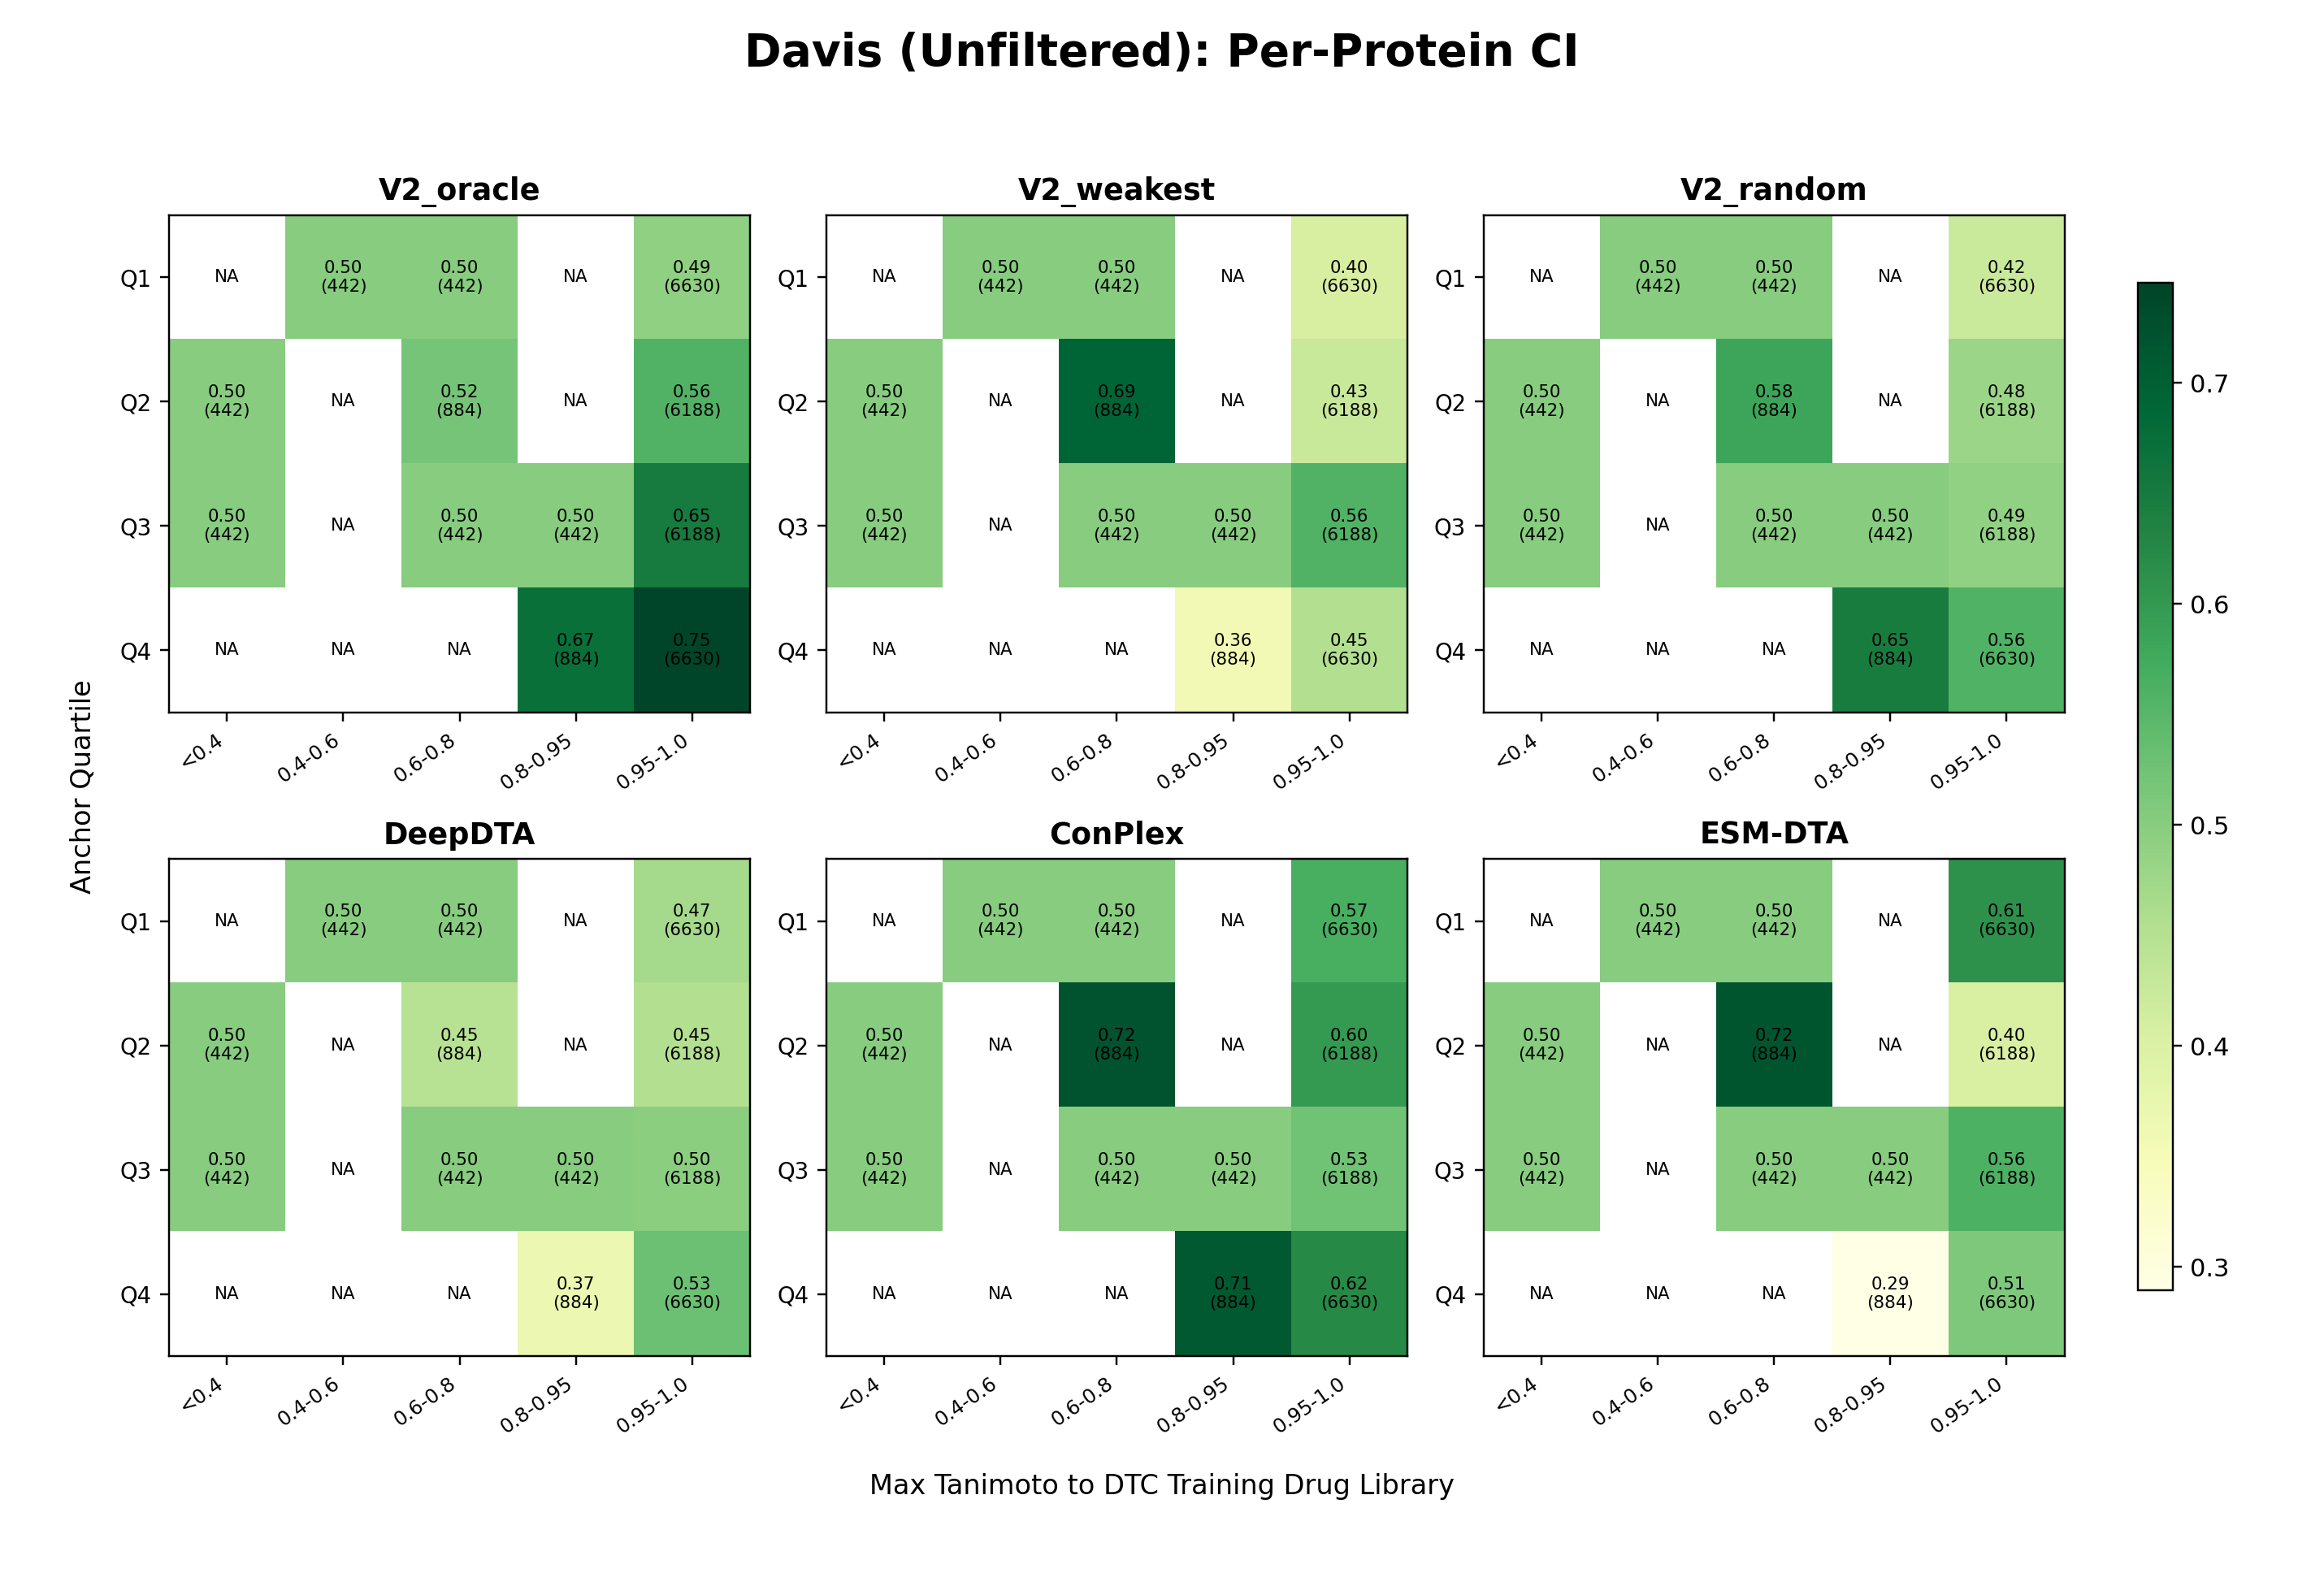
\includegraphics[width=\textwidth]{fig_davis_unfiltered_heatmap_ci.png}
        \caption{Davis, unfiltered}
    \end{subfigure}\hfill
    \begin{subfigure}[t]{0.49\textwidth}
        \centering
        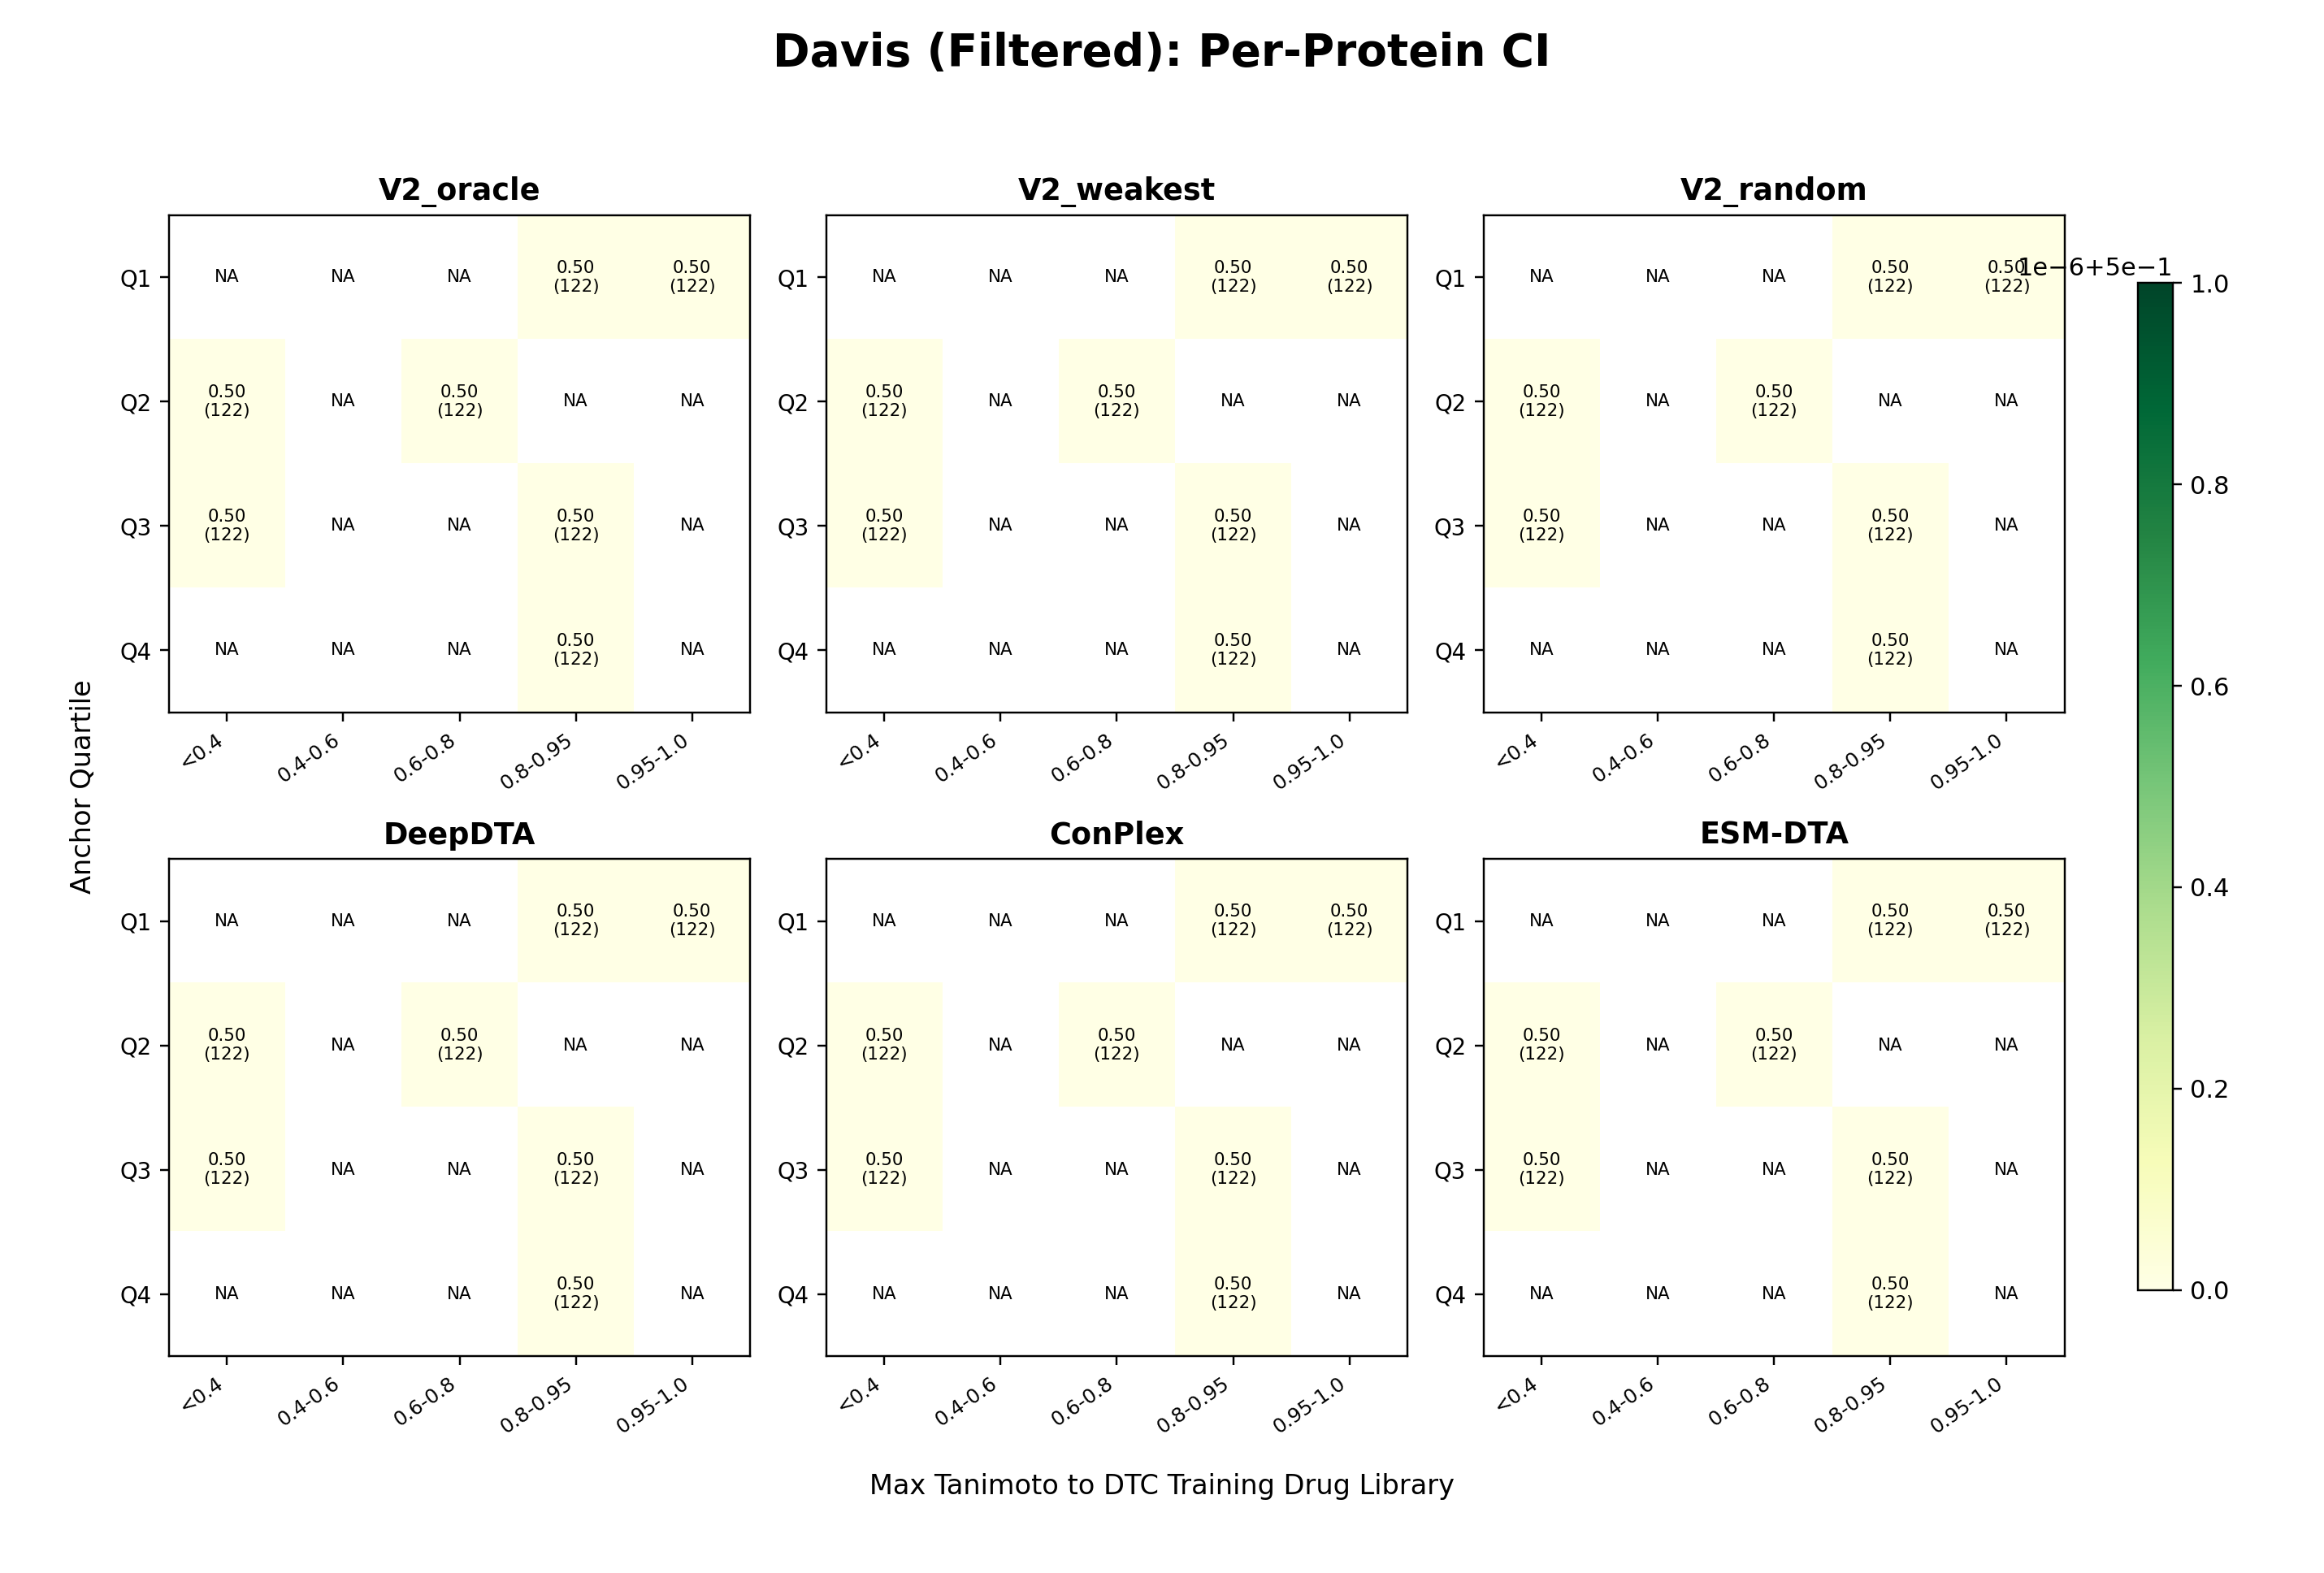
\includegraphics[width=\textwidth]{fig_davis_filtered_heatmap_ci.png}
        \caption{Davis, filtered}
    \end{subfigure}

    \vspace{0.8em}

    \begin{subfigure}[t]{0.49\textwidth}
        \centering
        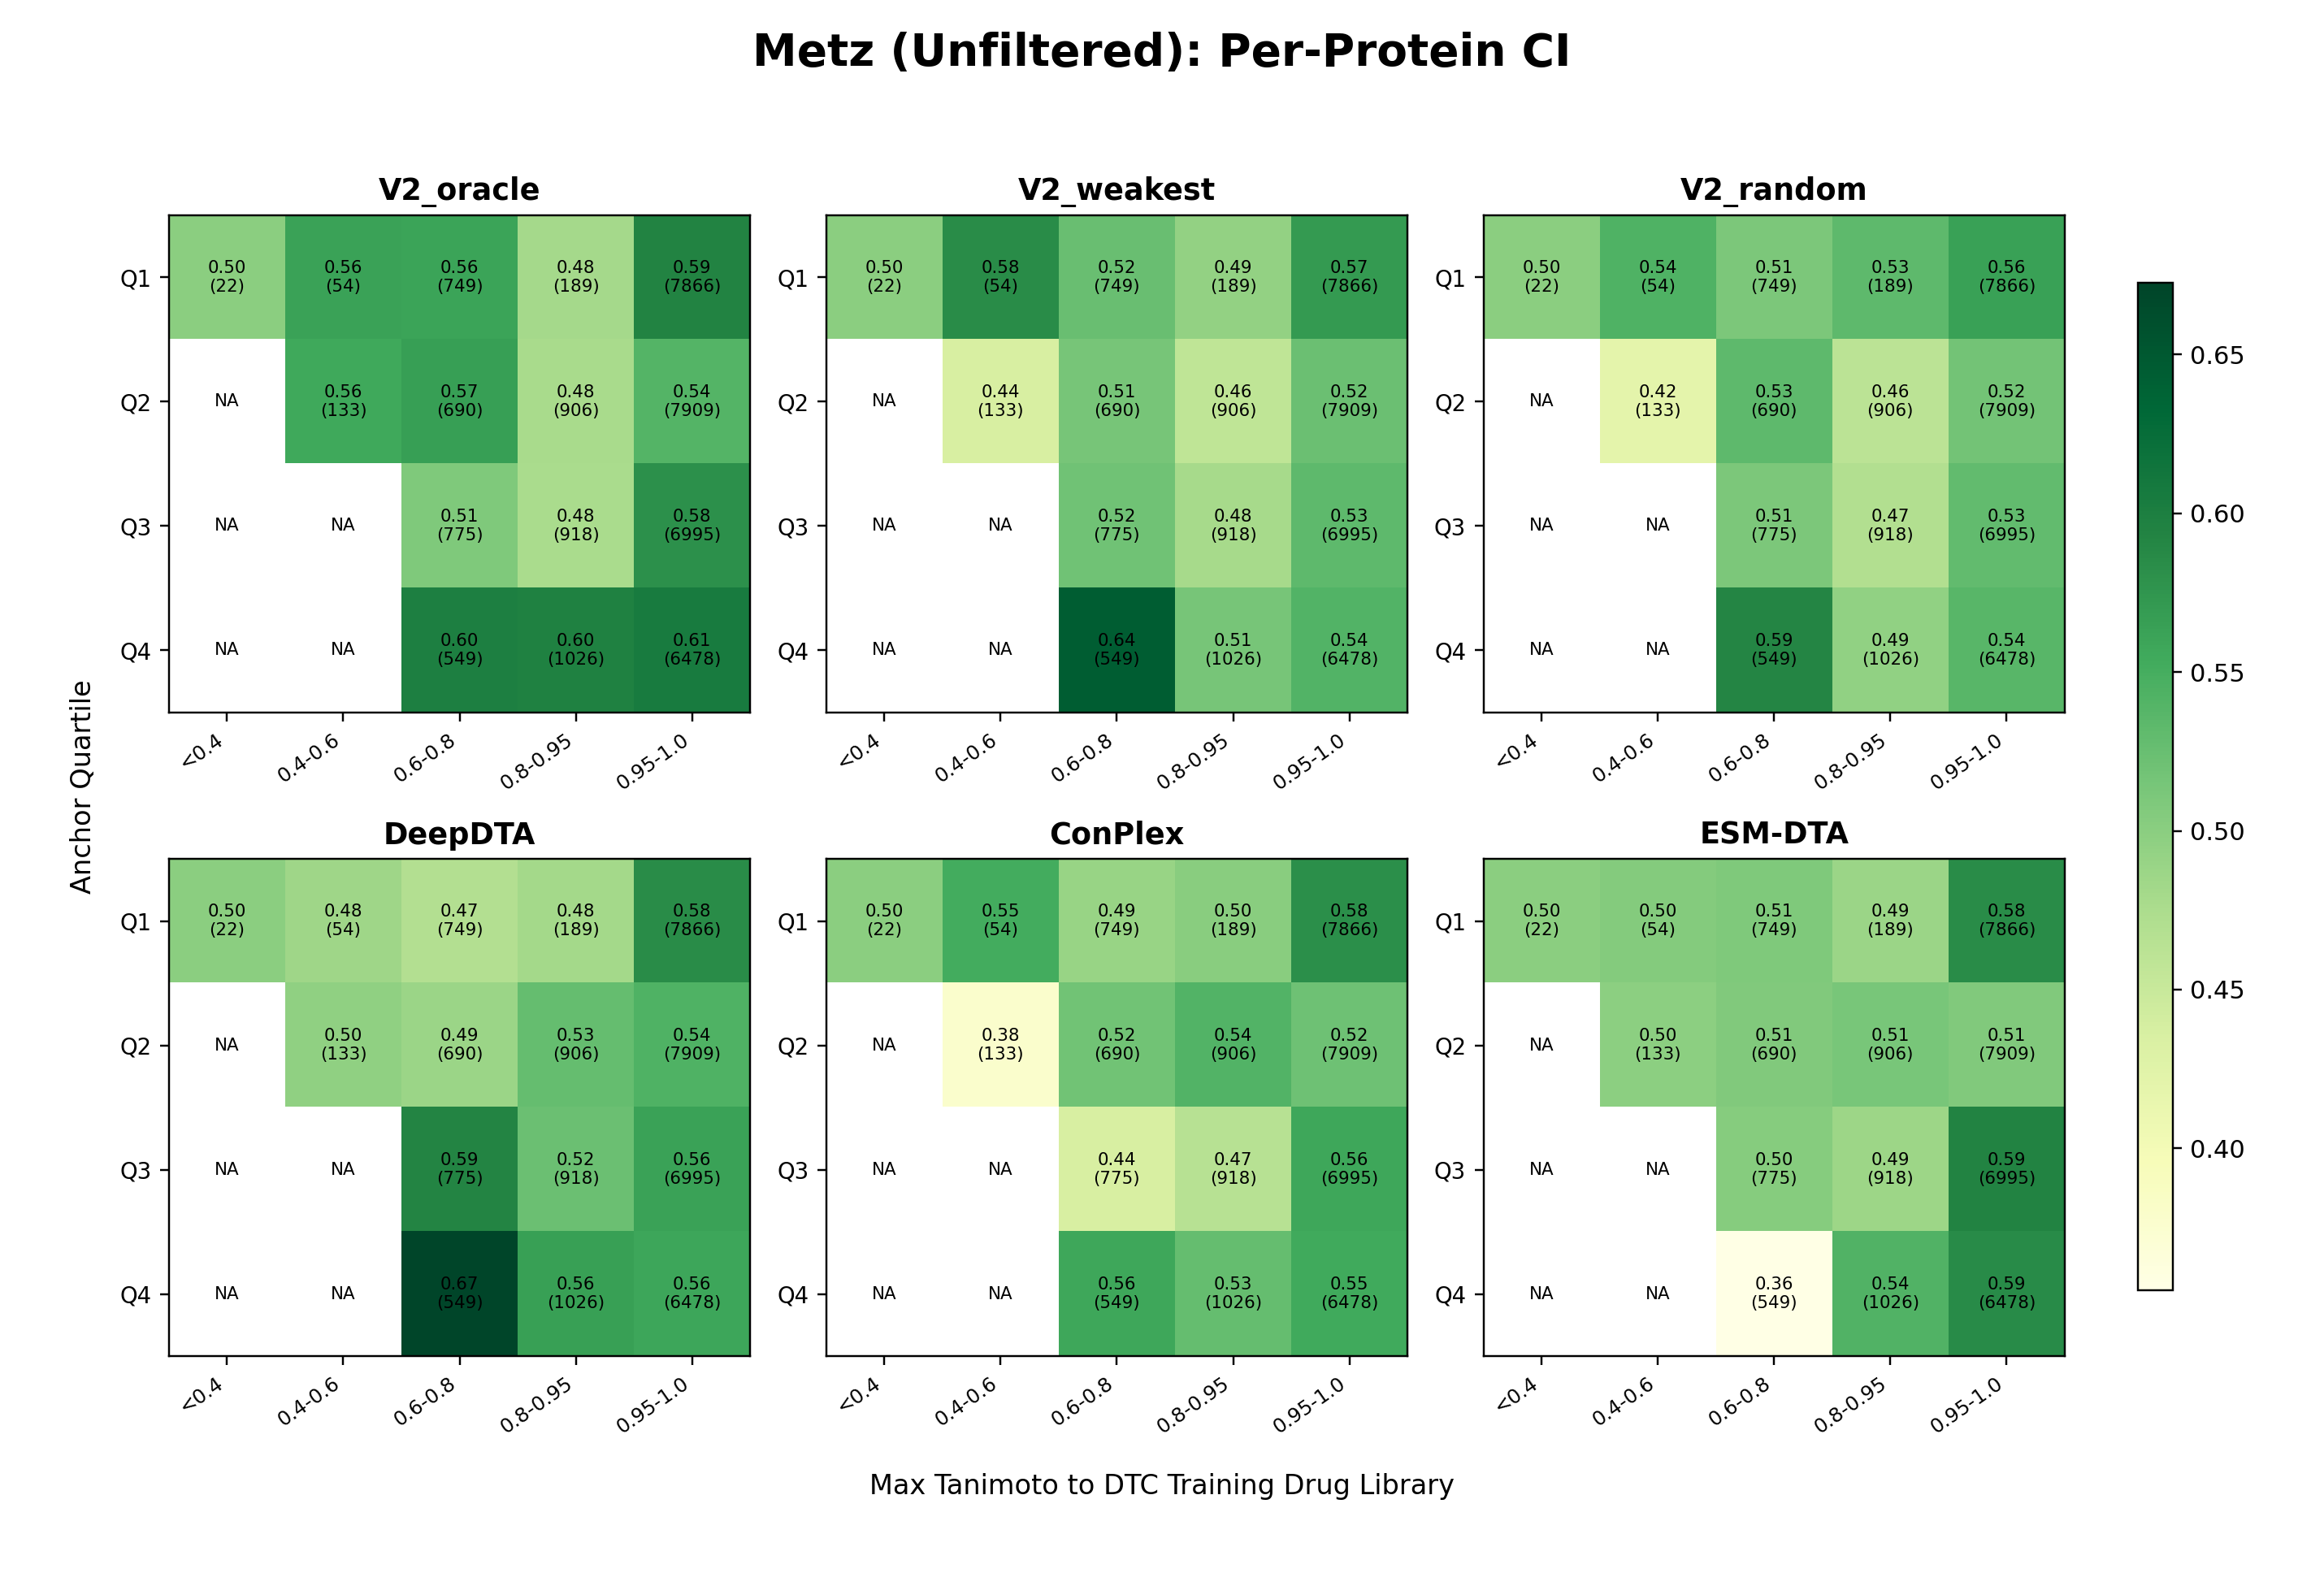
\includegraphics[width=\textwidth]{fig_metz_unfiltered_heatmap_ci.png}
        \caption{Metz, unfiltered}
    \end{subfigure}\hfill
    \begin{subfigure}[t]{0.49\textwidth}
        \centering
        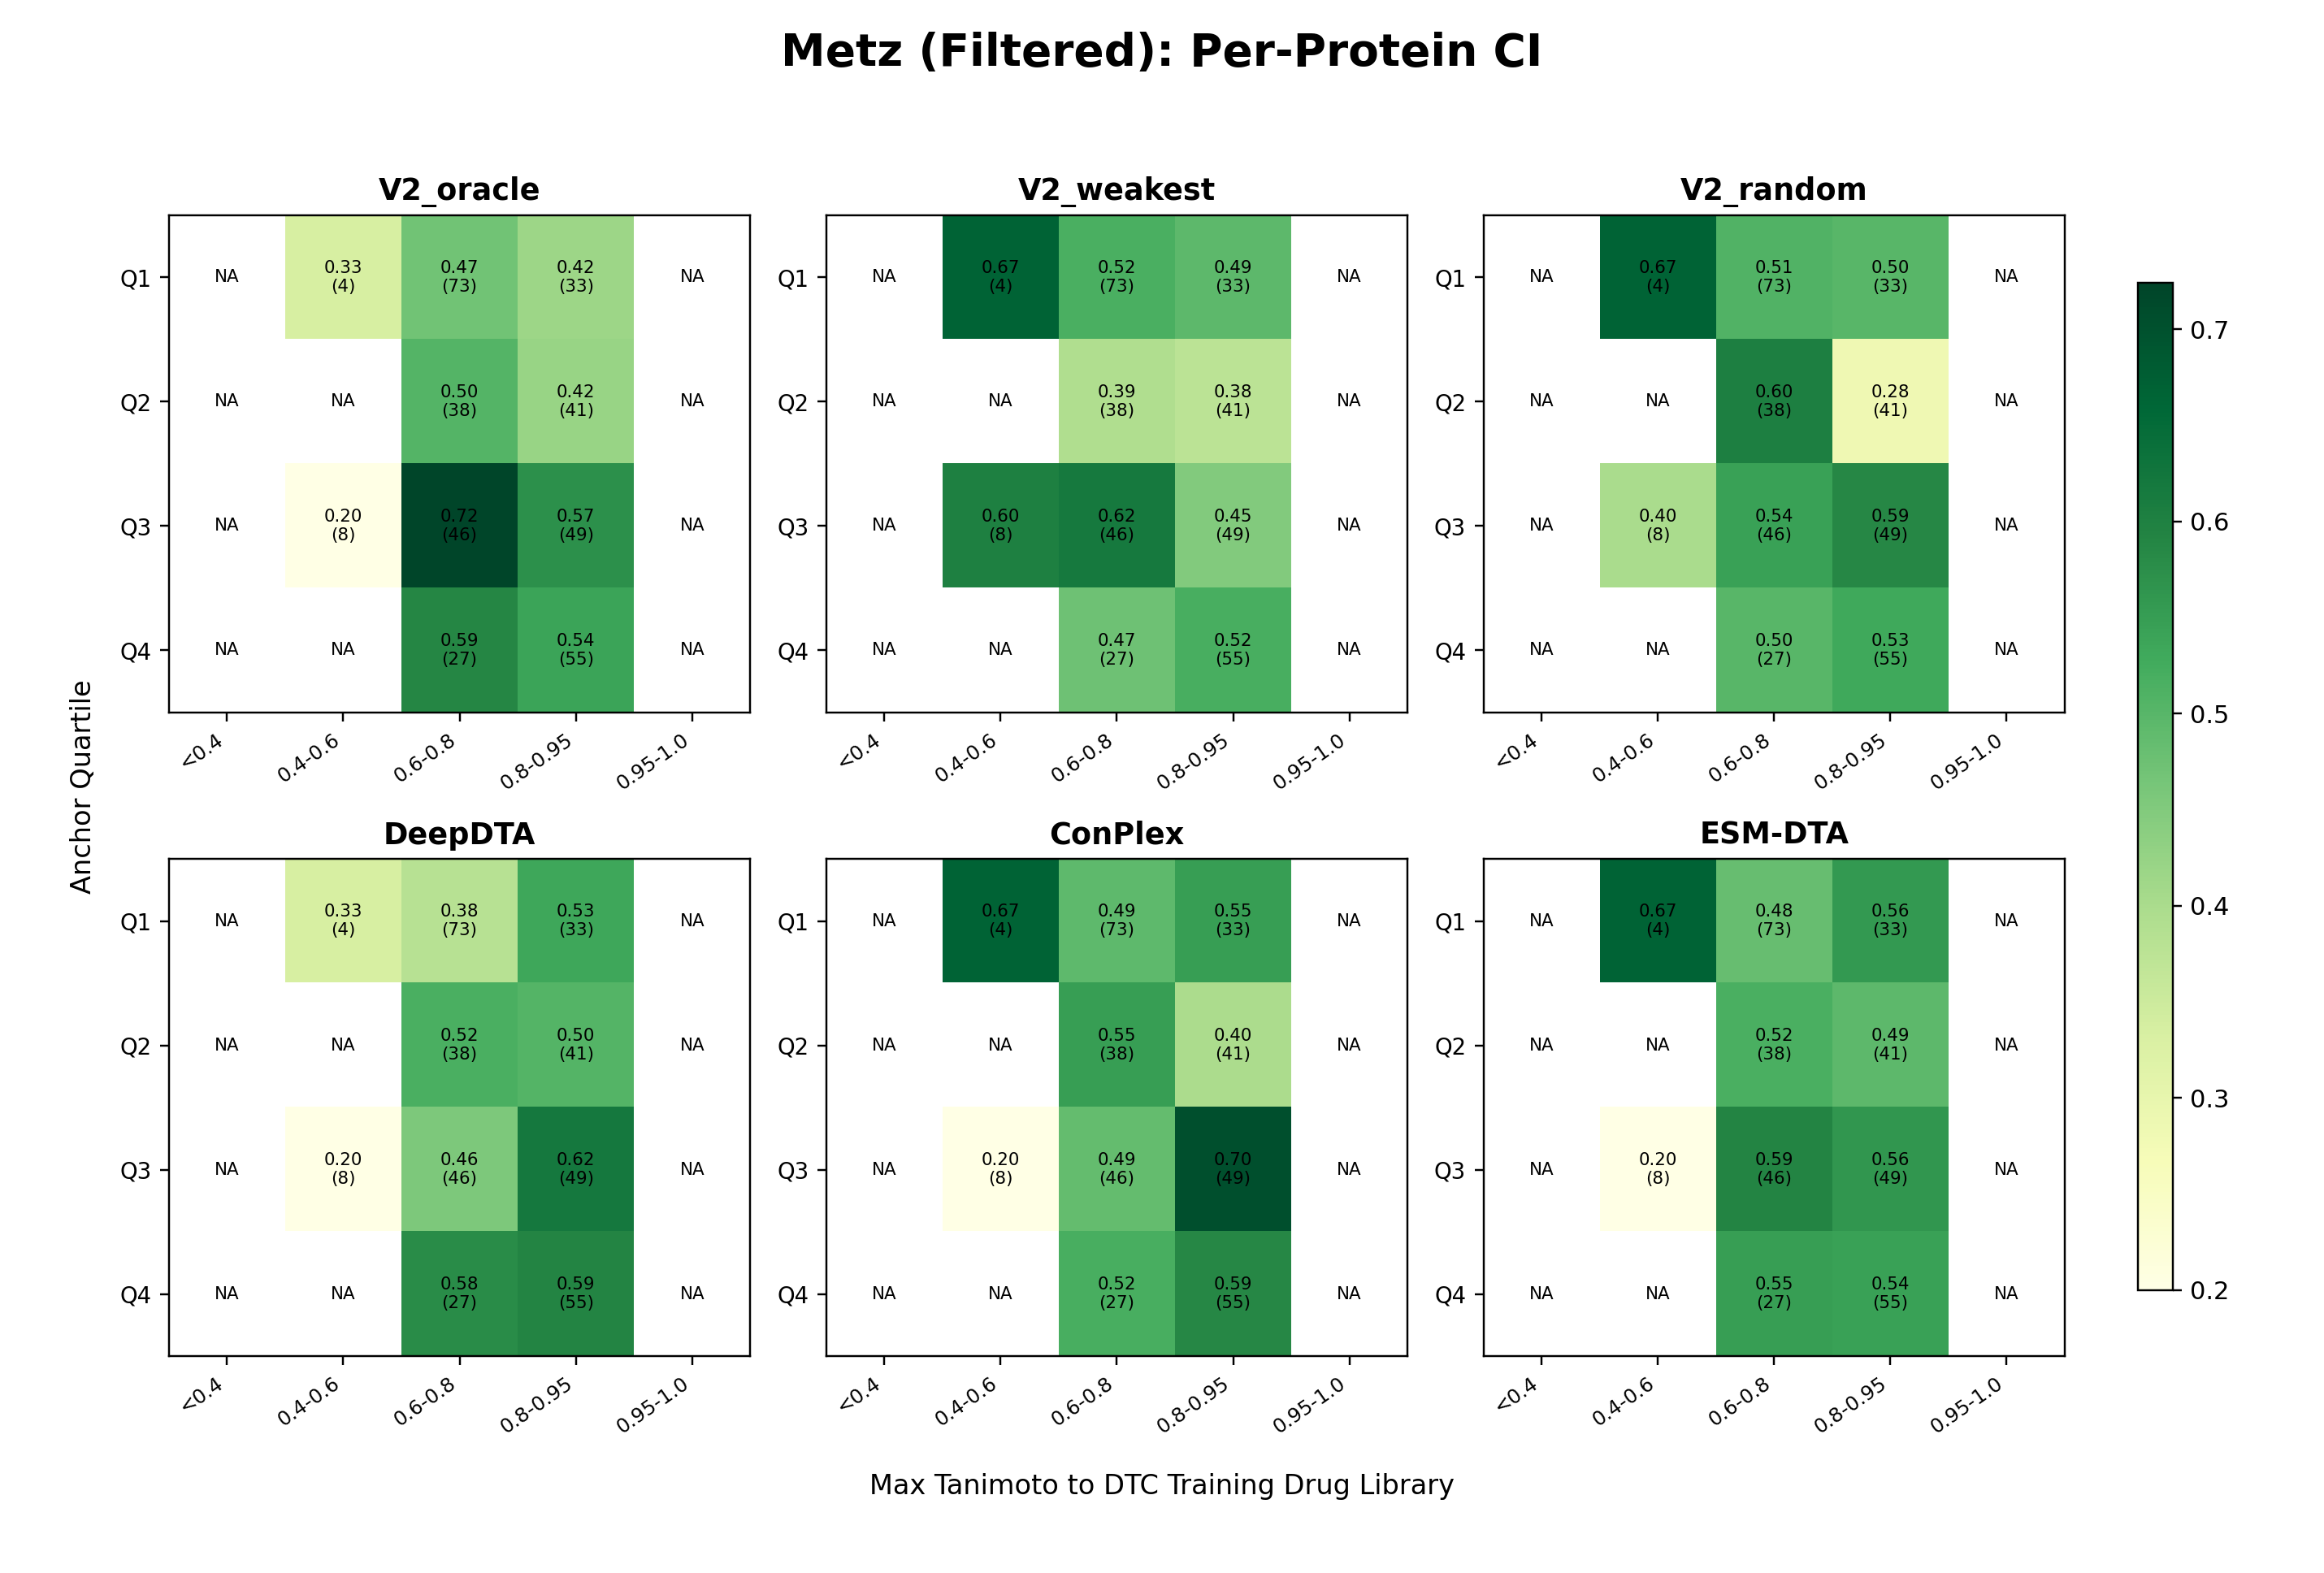
\includegraphics[width=\textwidth]{fig_metz_filtered_heatmap_ci.png}
        \caption{Metz, filtered}
    \end{subfigure}
    \caption{Per-protein mean CI heatmaps stratified jointly by anchor pKi quartile and maximum Tanimoto similarity to the DTC training drug library. The top row shows Davis before and after overlap filtering; the bottom row shows the same comparison for Metz. Each panel compares V2 oracle/weakest/random controls against DeepDTA, ConPlex*, and ESM-DTA. Numbers in cells indicate mean per-protein CI with the number of interactions in parentheses. The unfiltered panels reflect nominal benchmark difficulty, whereas the filtered panels expose how strongly the conclusions depend on overlap control.}
    \label{fig:benchmark_heatmaps_main}
\end{figure}

\begin{figure}[t]
    \centering
    \begin{subfigure}[t]{0.49\textwidth}
        \centering
        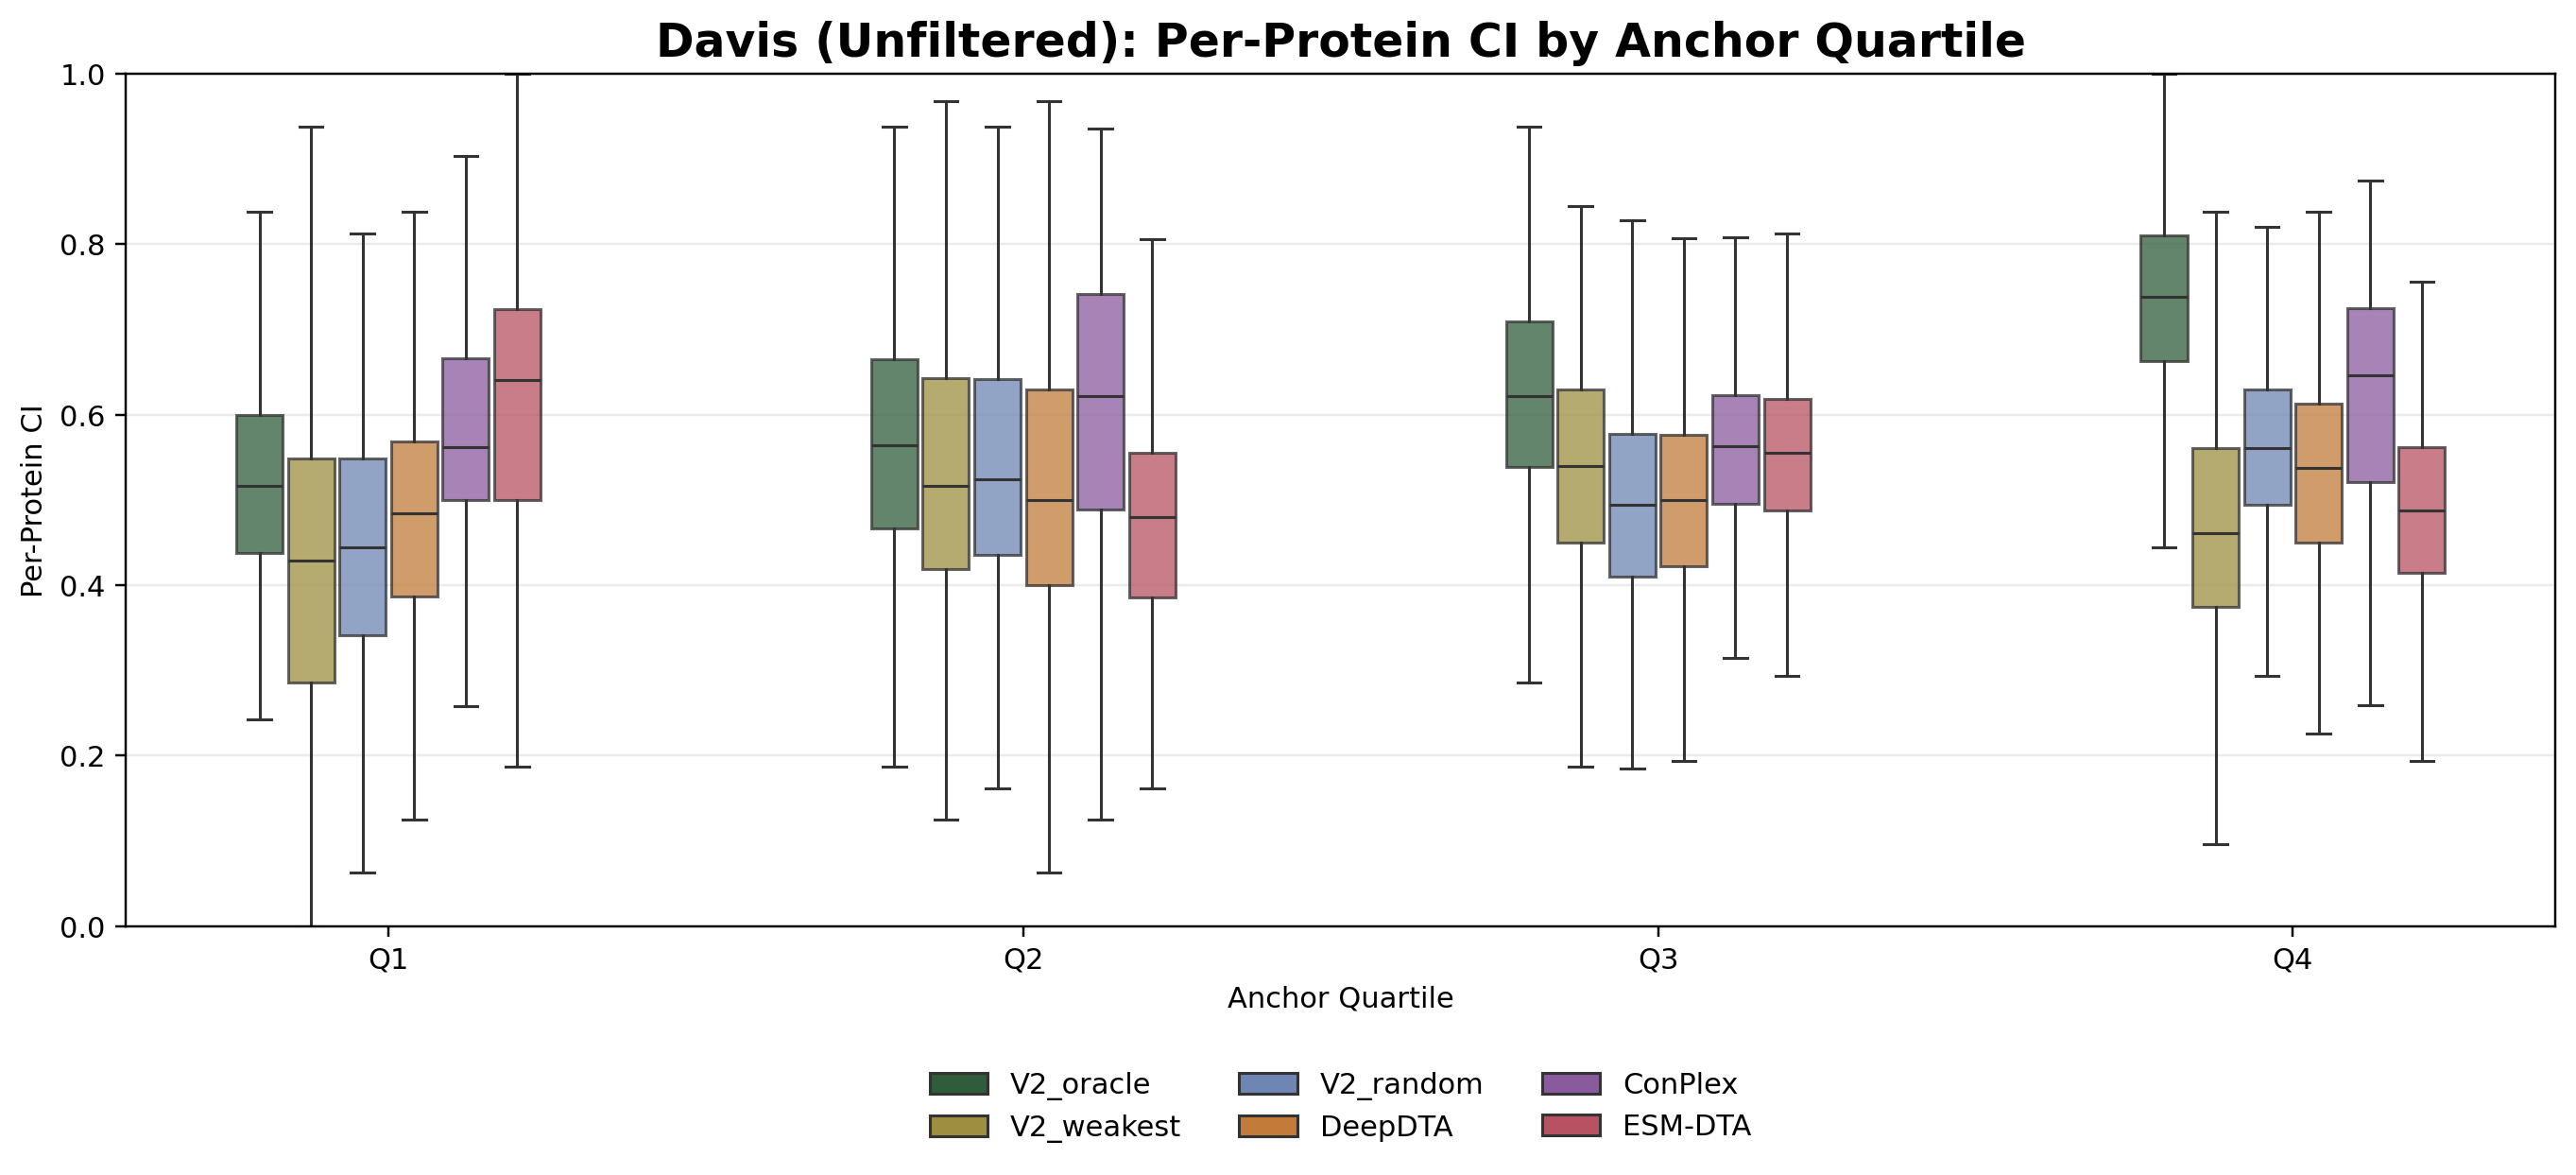
\includegraphics[width=\textwidth]{fig_davis_unfiltered_quartile_ci_distribution.png}
        \caption{Davis, unfiltered}
    \end{subfigure}\hfill
    \begin{subfigure}[t]{0.49\textwidth}
        \centering
        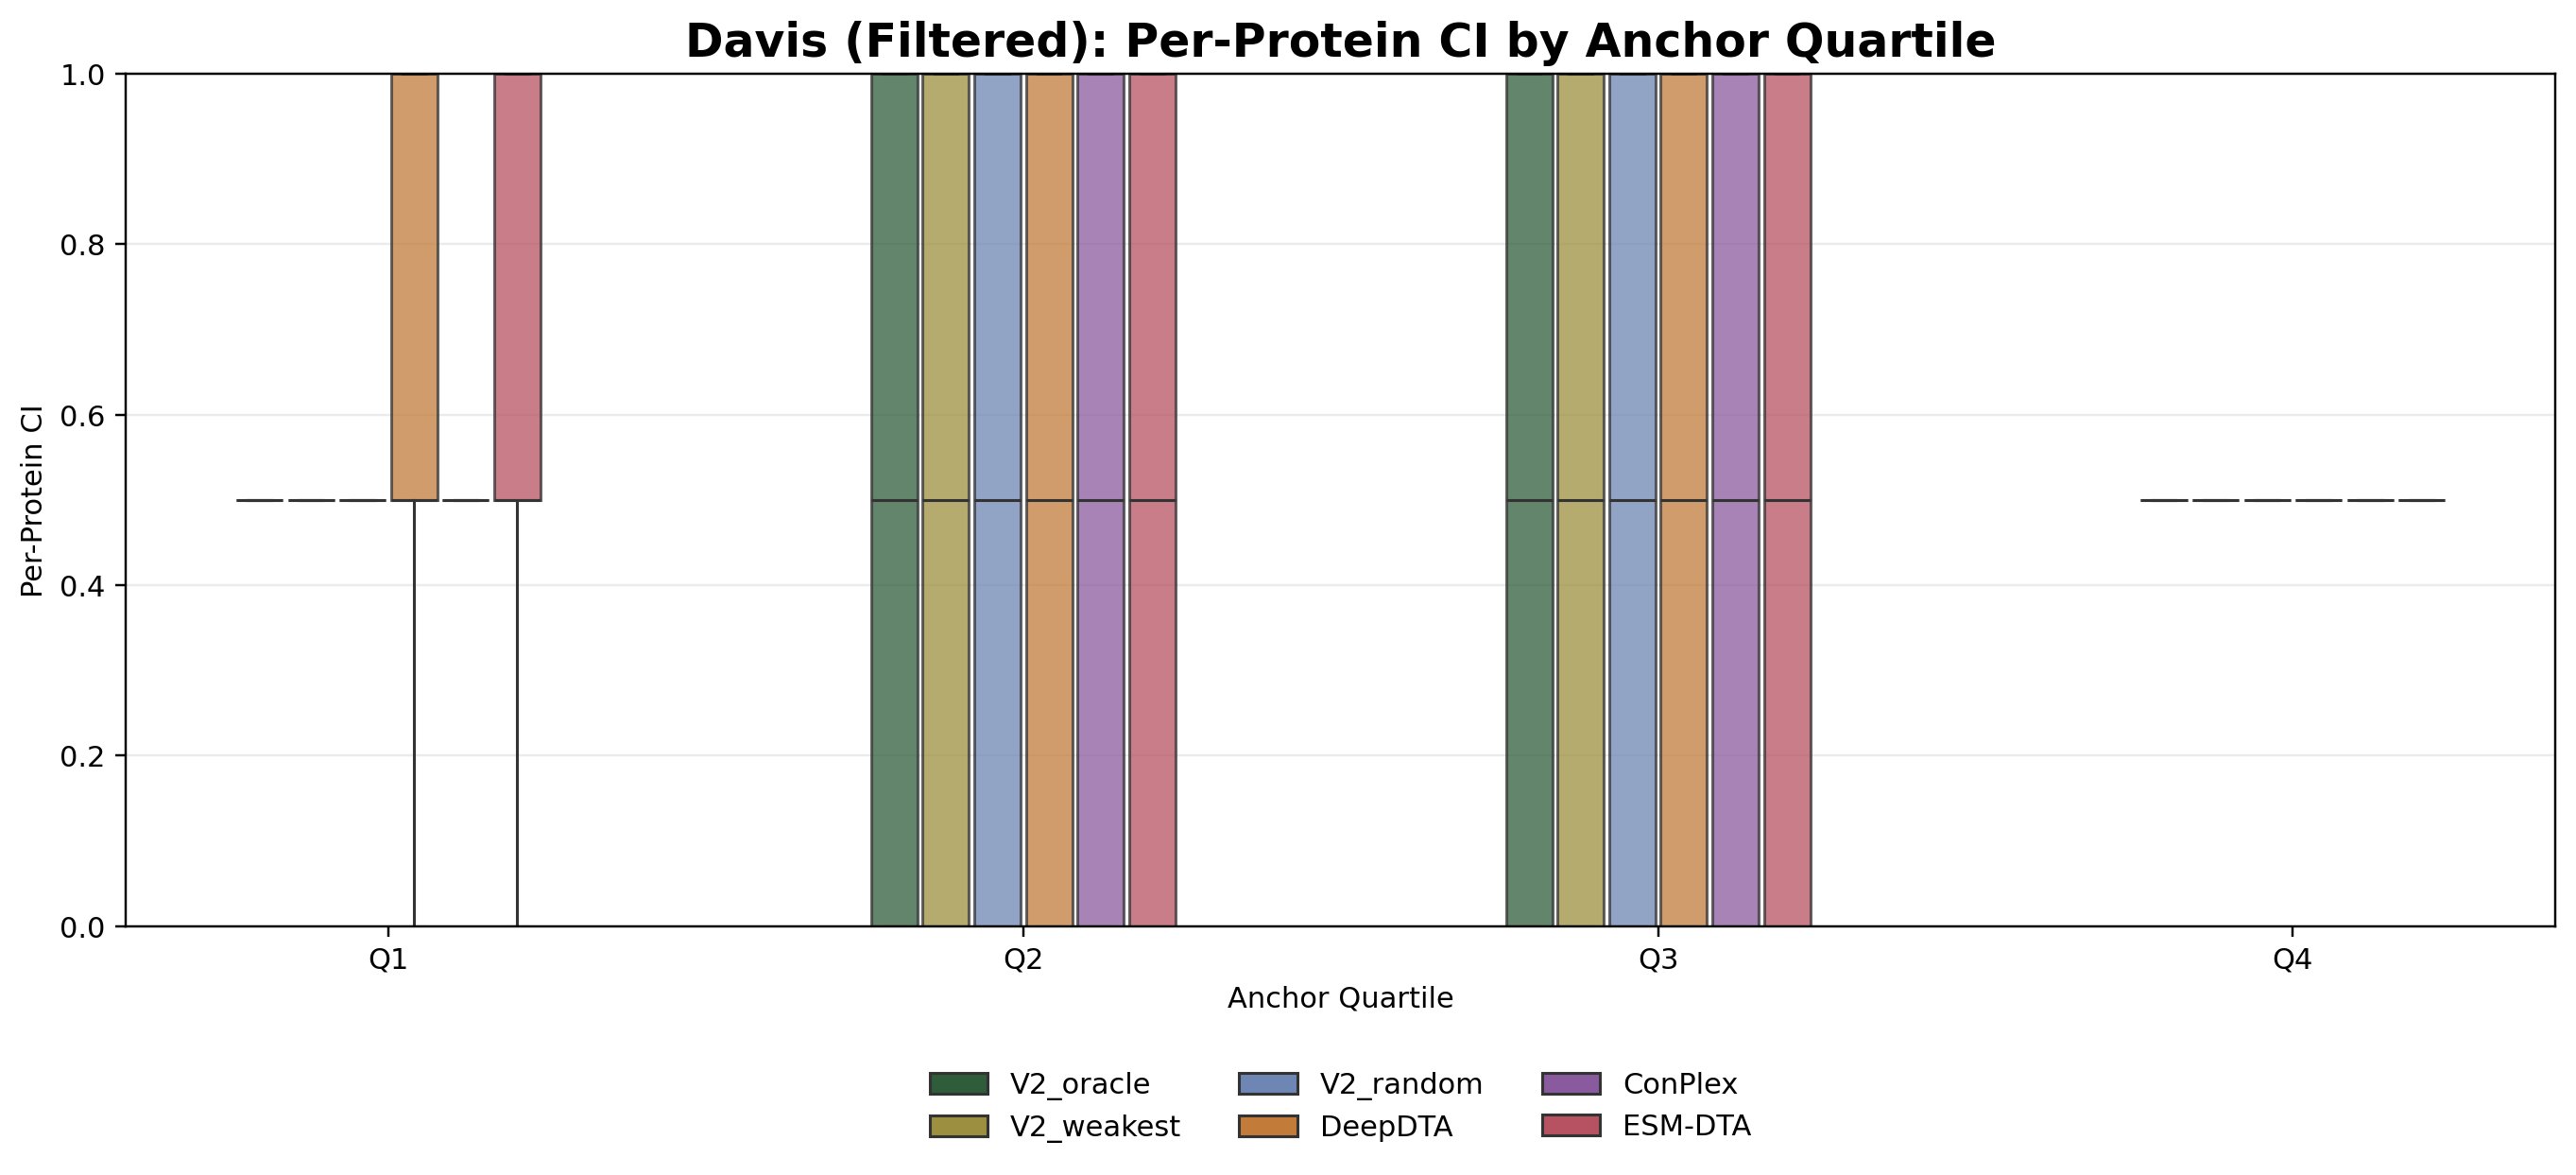
\includegraphics[width=\textwidth]{fig_davis_filtered_quartile_ci_distribution.png}
        \caption{Davis, filtered}
    \end{subfigure}

    \vspace{0.8em}

    \begin{subfigure}[t]{0.49\textwidth}
        \centering
        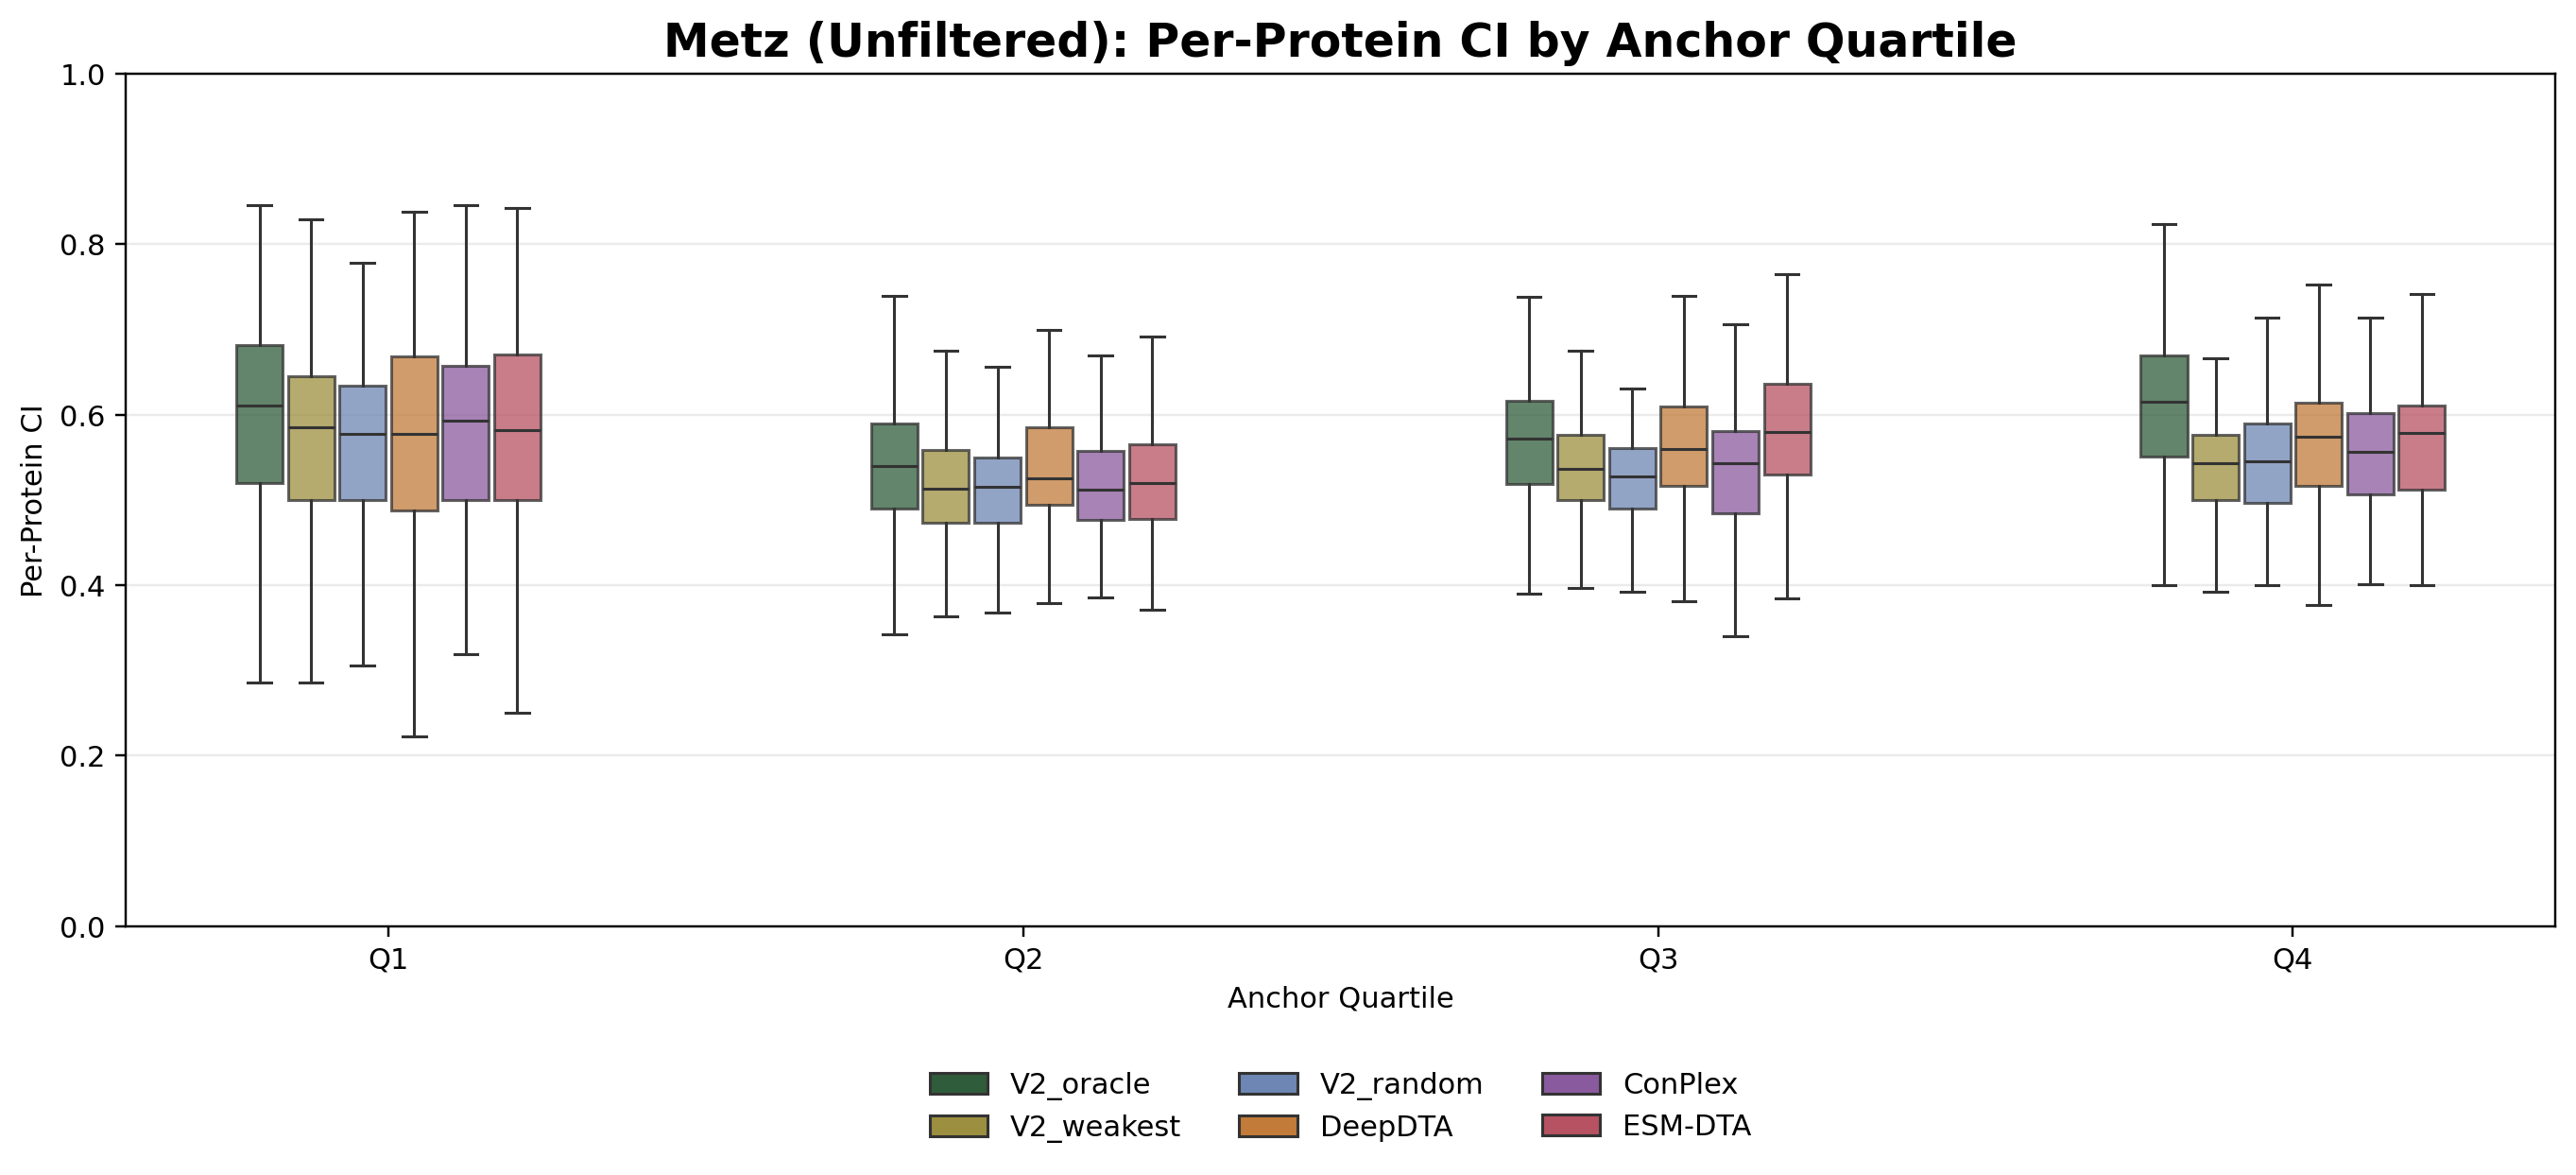
\includegraphics[width=\textwidth]{fig_metz_unfiltered_quartile_ci_distribution.png}
        \caption{Metz, unfiltered}
    \end{subfigure}\hfill
    \begin{subfigure}[t]{0.49\textwidth}
        \centering
        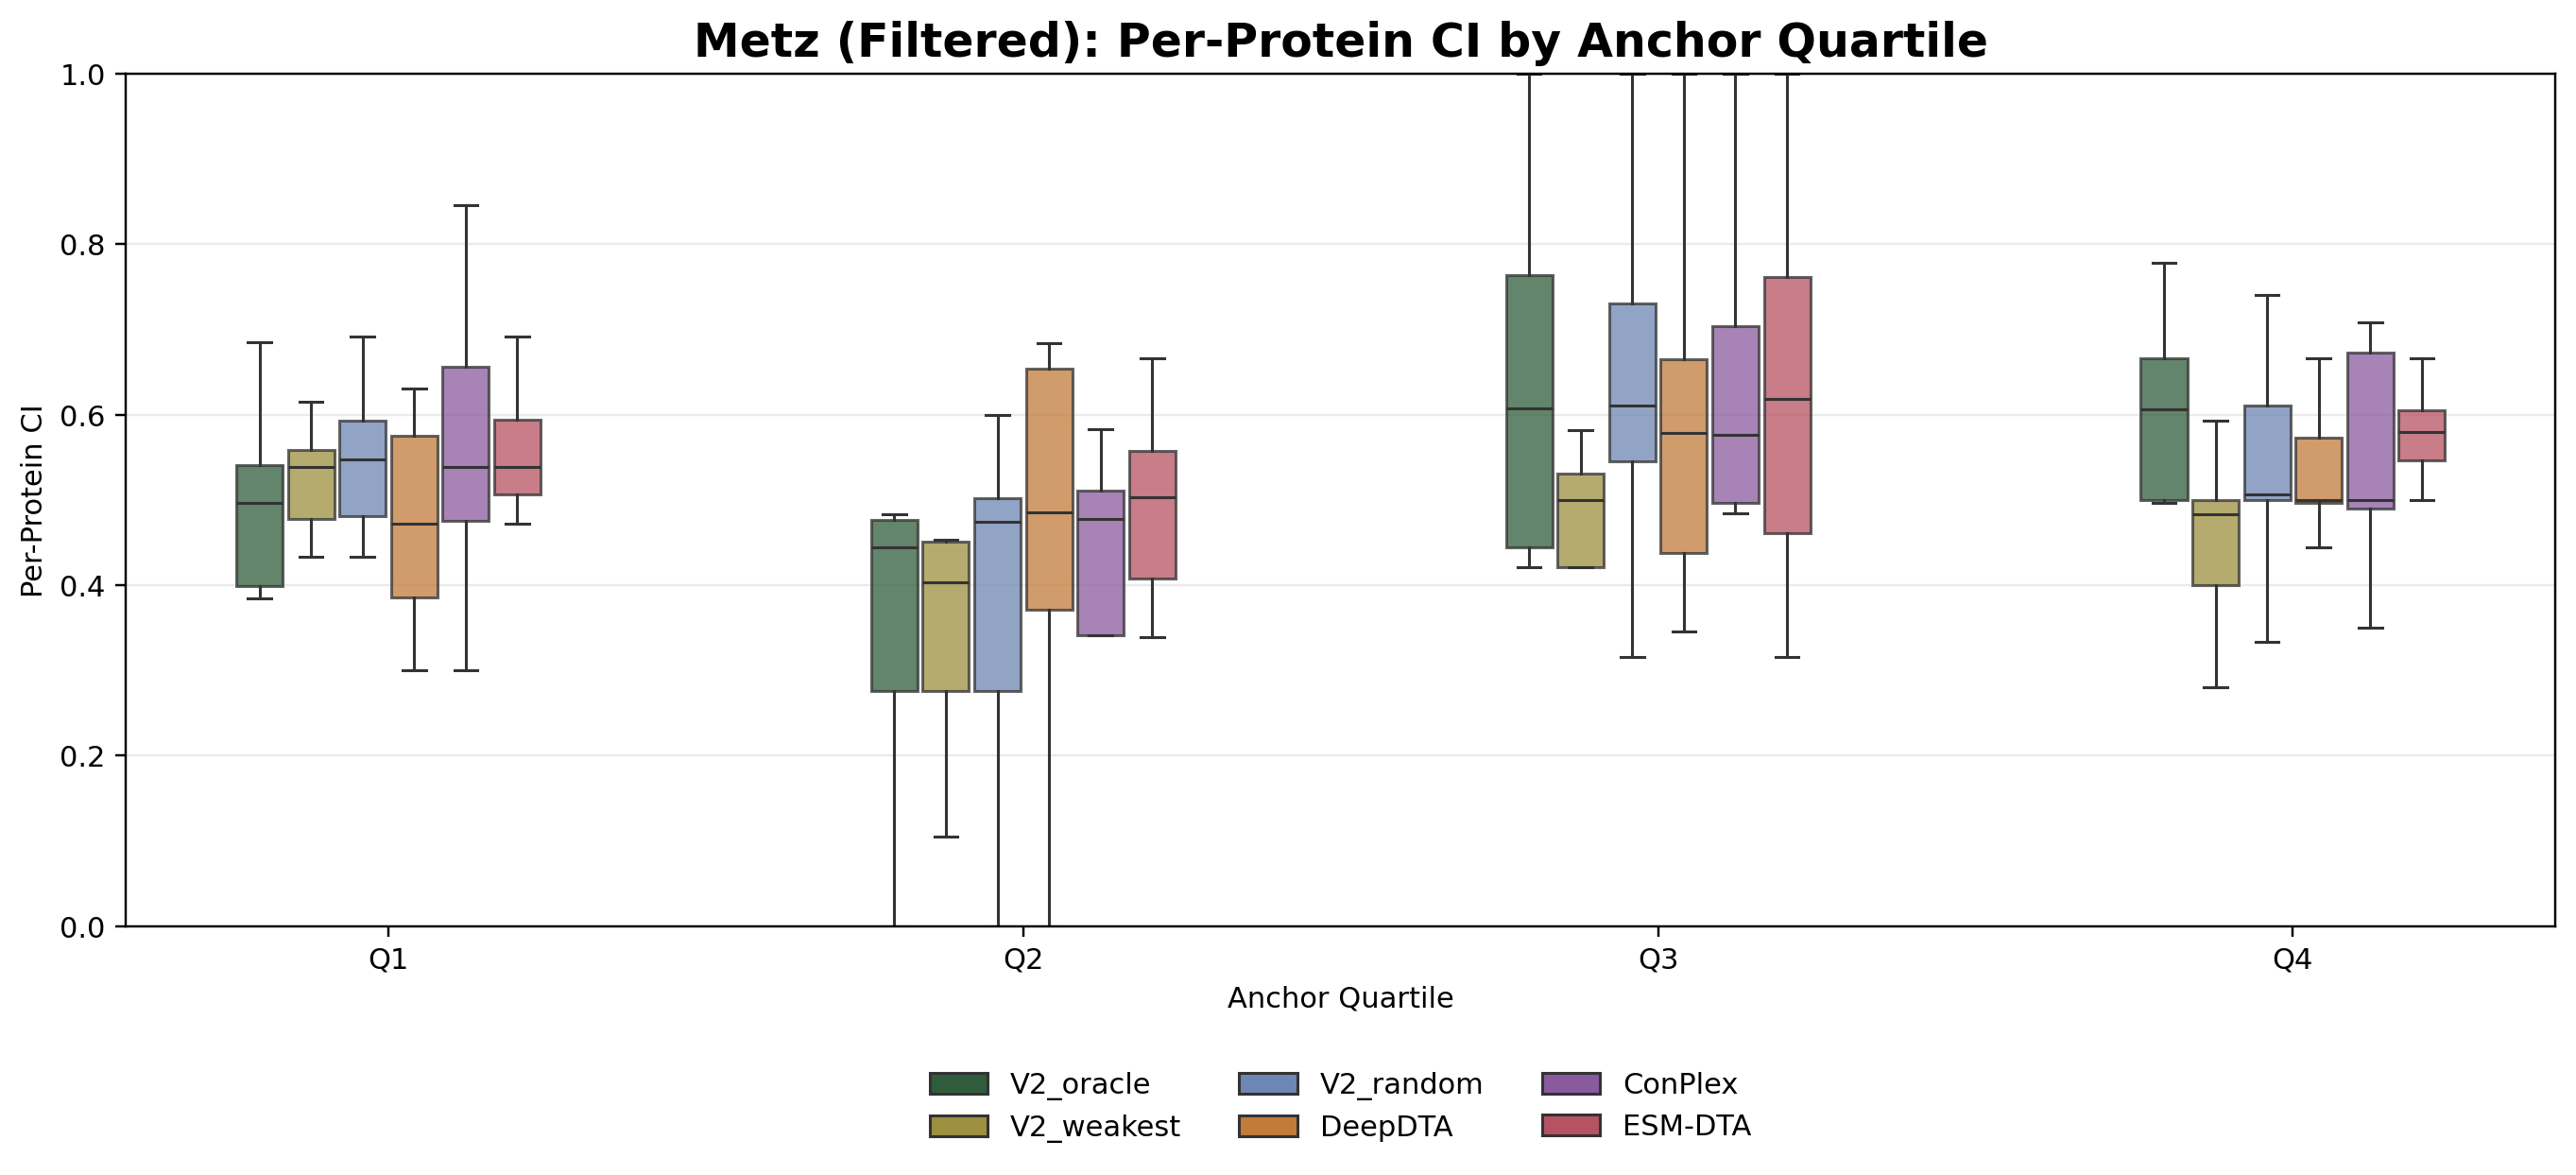
\includegraphics[width=\textwidth]{fig_metz_filtered_quartile_ci_distribution.png}
        \caption{Metz, filtered}
    \end{subfigure}
    \caption{Quartile-wise per-protein CI distributions under the same paired protocols. The unfiltered panels show the benchmark as typically reported, while the filtered panels remove protein and chemical overlap with the DTC training reference. This makes the regime change visible directly in the distributions: unfiltered Metz compresses the methods into similar CI ranges, whereas filtered Metz widens the gap in favor of V2-oracle; Davis remains more separated across anchor quartiles in both protocols, but the filtered view is much smaller and chemically narrower.}
    \label{fig:benchmark_quartile_dists_main}
\end{figure}

\subsection{Ablation: ESM-2 Scaling and Baseline Controls}

The ablations reveal that the transfer mechanism is sensitive to protein encoder scale (Figure~\ref{fig:esm_scaling}). Scaling from ESM-2 35M to 650M improves Davis performance (AUROC 0.669 versus 0.644, CI 0.642 versus 0.605). The larger model captures richer protein representations that improve the anchor--query comparison.

\begin{figure}[t]
    \centering
    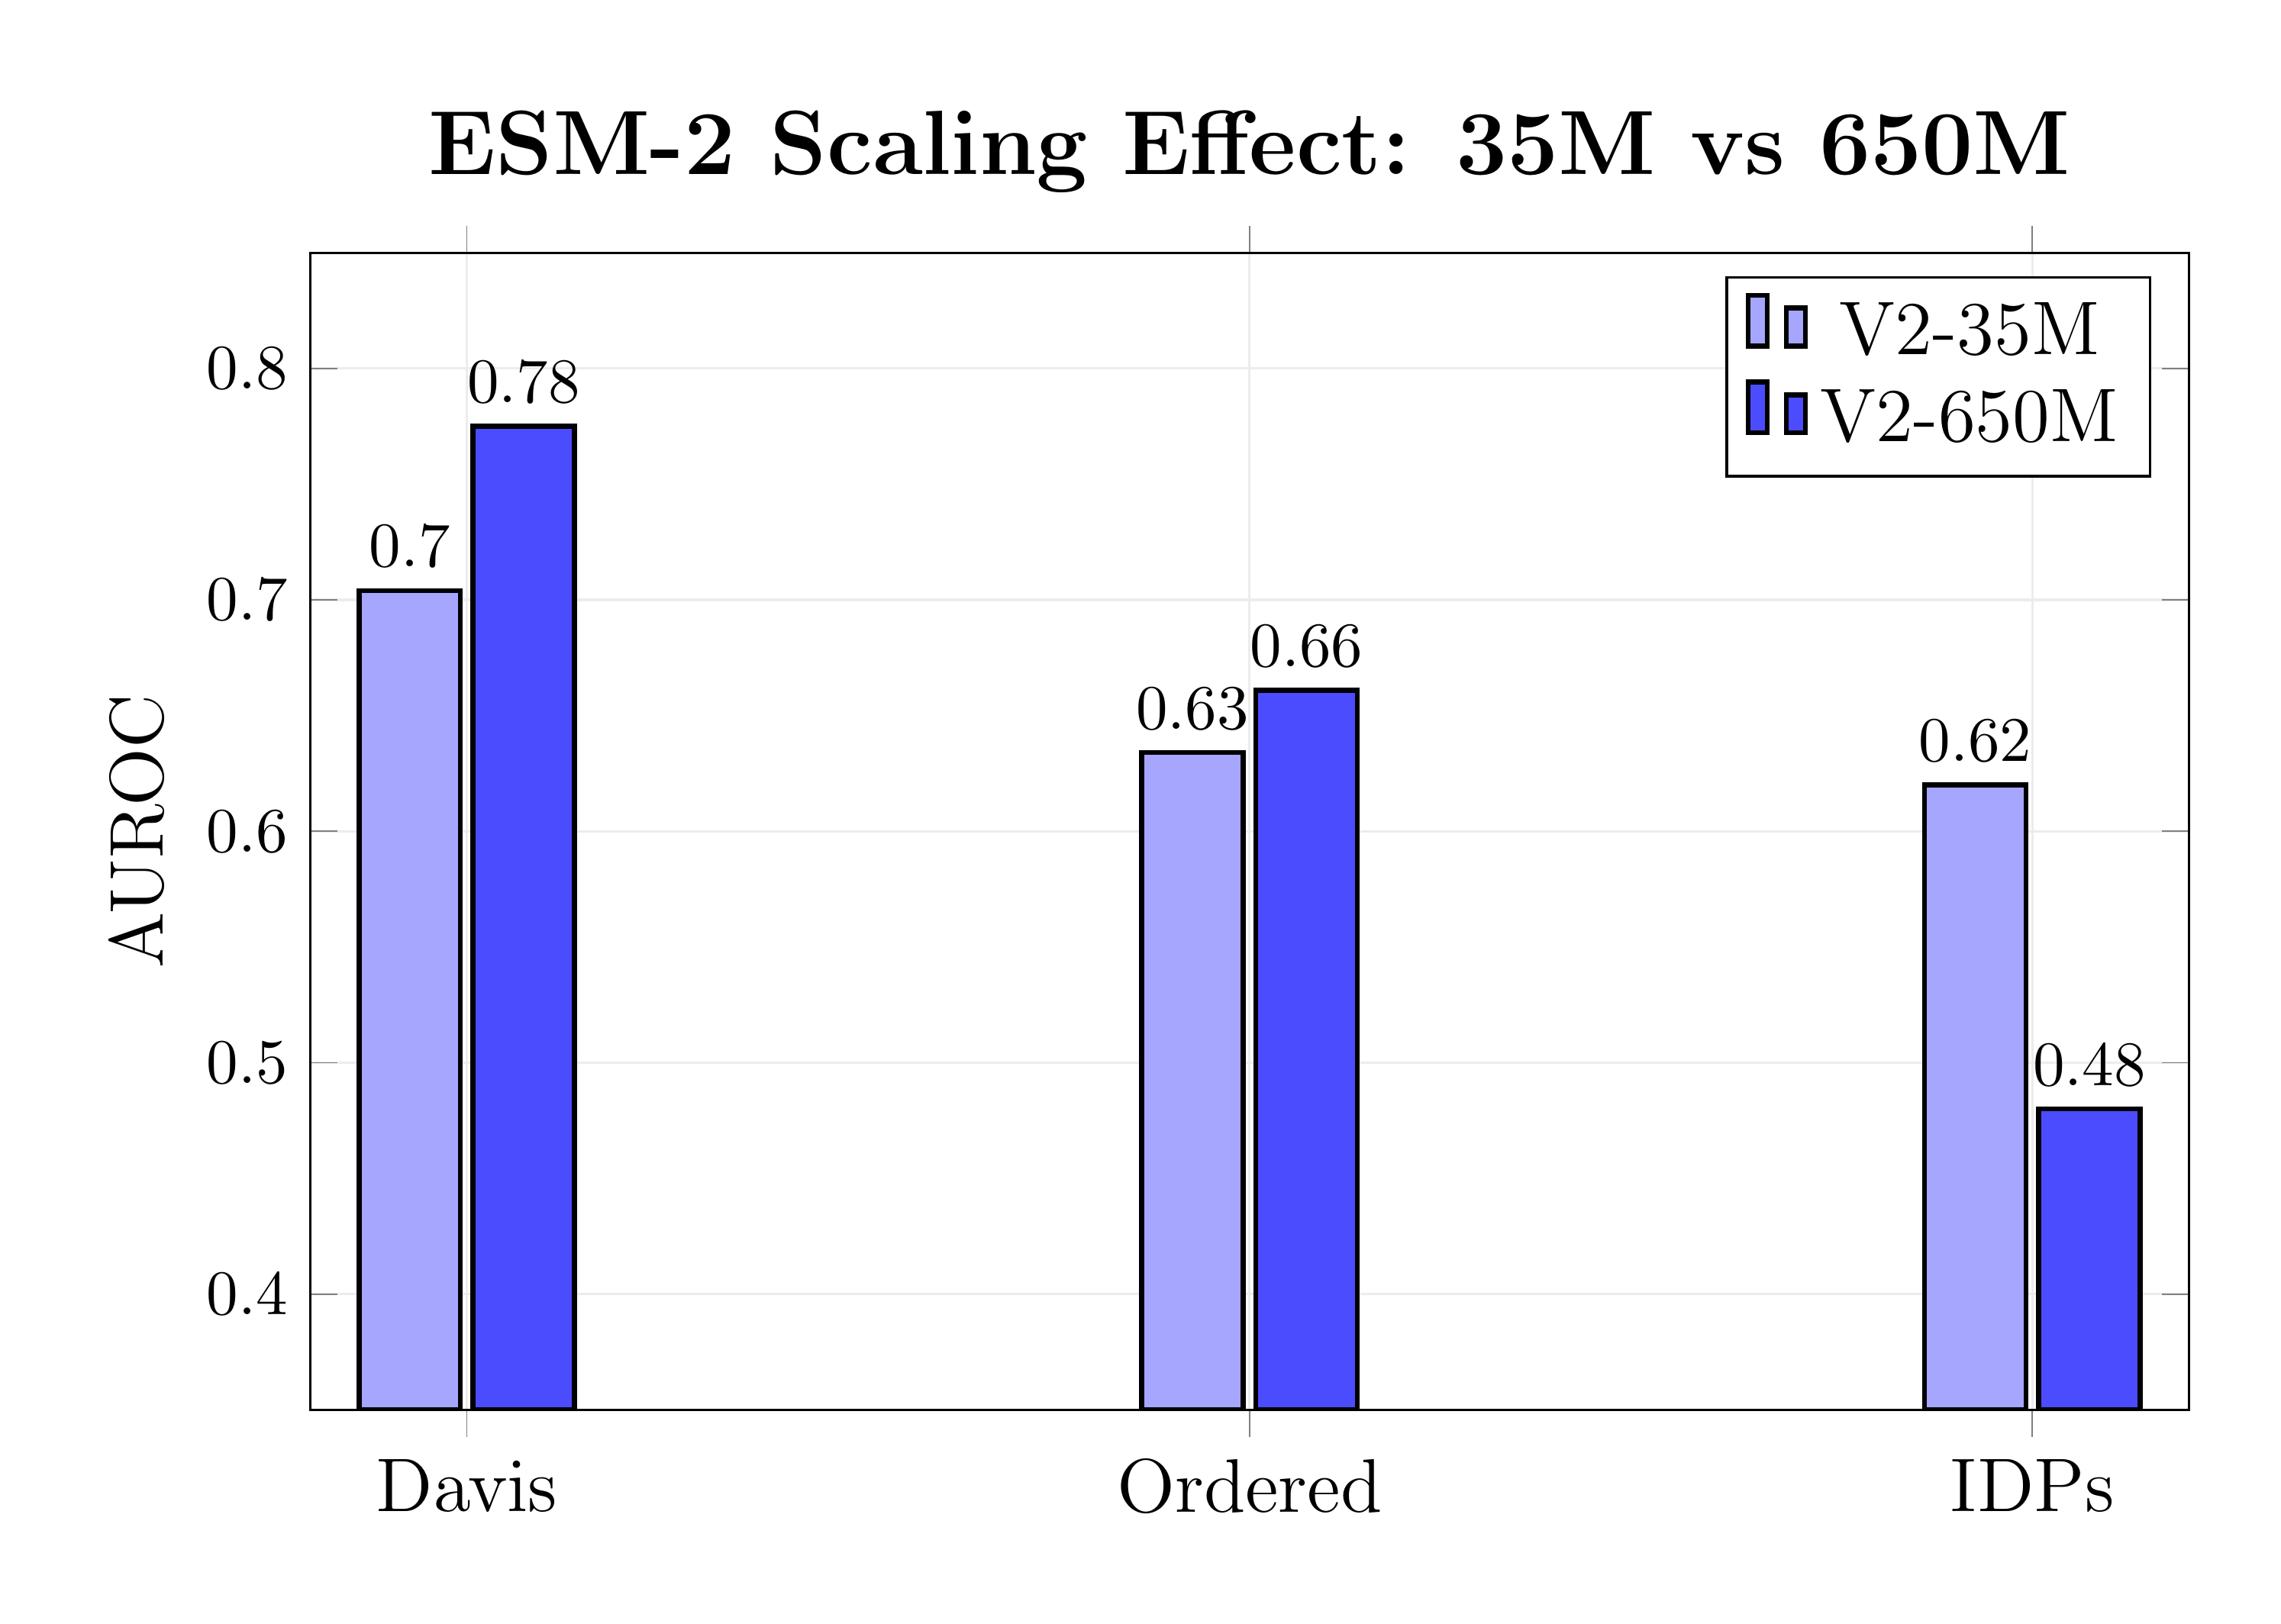
\includegraphics[width=0.75\textwidth]{fig7_esm_scaling.png}
    \caption{Effect of ESM-2 scaling (35M vs 650M parameters) on Davis cross-dataset transfer. The larger model improves performance across all anchor quartiles, with the largest gains on weak anchors (Q1--Q2).}
    \label{fig:esm_scaling}
\end{figure}

ESM-DTA serves as a negative control for the hypothesis that stronger protein embeddings alone are enough. It achieves the best same-dataset performance on DTC (AUROC 0.910, CI 0.707) but collapses on Davis (per-protein AUROC 0.503, CI 0.501---indistinguishable from random). The contrast between Table~\ref{tab:dtc_test} and Table~\ref{tab:davis_cross_dataset} indicates that the improvement does not come from ESM-2 alone. It comes from changing the prediction problem from isolated pair scoring to transfer from a known anchor.

\subsection{Secondary Controls: Drug-Side Anchors and Conformation Weighting}

Two secondary analyses help delimit what the anchor mechanism is, and is not, using as signal. First, the Drug-Anchor ablation reverses the modality of the support example by conditioning on a strong \emph{drug} for the same protein rather than a strong protein for the same drug. This variant remains competitive in-distribution (DTC test AUROC 0.906) and stays above pairwise baselines on several external benchmarks, but it does not match the main protein-anchor formulation on Davis (AUROC 0.559 in Figure~\ref{fig:cross_dataset}, versus 0.669 for V2-650M). This makes the ablation useful as a control rather than a replacement: the transfer idea is not protein-exclusive, but protein-side anchoring is the stronger direction for the kinase-focused cross-dataset setting studied here.

Second, a conformation-weighted negative control on the IDP benchmark asks whether structural proximity alone can explain the gain. Replacing the query ESM-2 embedding with a TM-score-weighted average of embeddings from structurally matched ordered proteins reduces AUROC from 0.584 to 0.575 on the common IDP subset ($n=2{,}442$). The result argues against a simple ``borrow a similar structure'' explanation. What transfers is not generic structural resemblance, but experimentally grounded binding context supplied by the anchor. Full architectural and protocol details for both controls are provided in the Supplementary Information.


\subsection{Anchor Quality Stratification on the Davis Kinase Benchmark}
\label{sec:anchor_quartile}

To understand how anchor binding strength affects prediction quality, we stratify the Davis kinase benchmark~\citep{davis2011kinase} by anchor pKi.
As described in Section~\ref{sec:cross_dataset}, anchors are retrieved from the DTC training set by Tanimoto chemical similarity, with a minimum anchor pKi of 7 (confirmed binders).
For the quartile analysis, we use the oracle anchor variant (strongest known binder per drug within Davis) to isolate the effect of anchor strength from retrieval quality; the main cross-dataset results in Table~\ref{tab:davis_cross_dataset} use realistic Tanimoto-retrieved anchors throughout.

\paragraph{Data characteristics.}
The Davis benchmark is a dense kinase selectivity panel: 442 kinases screened against 68 compounds, with binding measured as dissociation constant K$_d$.
The resulting pKd distribution is highly skewed: 91.4\% of interactions have pKd $< 7$ (non-binders at the assay sensitivity floor of pKd $= 5.0$), with only 2,500 of 29,170 pairs qualifying as true binders (pKd $\geq 7$).
This extreme class imbalance makes Davis a stringent test of binding discrimination---models must distinguish the 8.6\% true binders from a large background of non-binding kinases.

The oracle anchor pKi distribution is narrow (mean $9.10 \pm 0.70$, range 7.0--10.8) because each drug's strongest binder is typically a high-affinity kinase.
Anchor reuse is heavy: only 85 unique anchor proteins serve 29,170 interaction pairs, with a single kinase (DDR1) acting as anchor for 1,766 pairs (6.1\%).
This reflects the kinase family's shared structural fold---a small number of promiscuous kinases bind most compounds strongly.

Figure~\ref{fig:davis_distribution} shows the target pKi distribution, anchor pKi distribution, binder fraction per quartile, and interaction counts per quartile.

\begin{figure}[t]
    \centering
    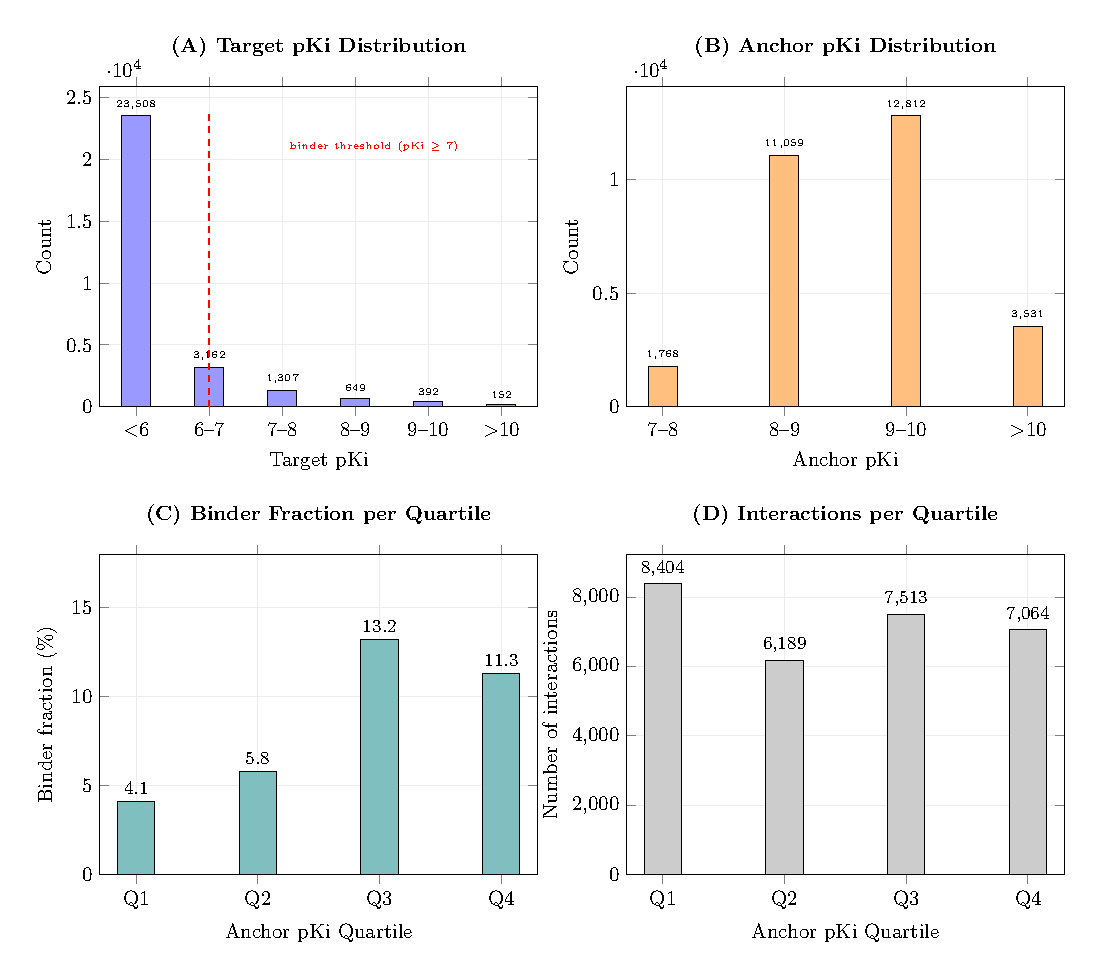
\includegraphics[width=\textwidth]{fig_davis_distribution.pdf}
    \caption{Davis benchmark data characteristics. \textbf{(A)}~Target pKi distribution: 91.4\% of interactions are non-binders (pKi $< 7$), concentrated at the assay floor of pKd $= 5.0$. \textbf{(B)}~Anchor pKi distribution (anchors $\geq 7$ only): most anchors have pKi 8--10. \textbf{(C)}~Binder fraction per anchor quartile: Q3 has the highest binder rate (13.2\%) despite not having the strongest anchors. \textbf{(D)}~Interaction counts per quartile, with the number of unique anchor proteins annotated.}
    \label{fig:davis_distribution}
\end{figure}

\paragraph{Quartile definition.}
We partition the 29,170 interactions into four quartiles by anchor pKi: Q1 (7.0--8.7, $n = 8{,}404$, 41 anchors), Q2 (8.7--9.1, $n = 6{,}189$, 23 anchors), Q3 (9.1--9.5, $n = 7{,}513$, 27 anchors), and Q4 (9.6--10.8, $n = 7{,}064$, 20 anchors).
The binder fraction increases from Q1 (4.1\%) to Q3 (13.2\%) before declining slightly in Q4 (11.3\%), reflecting the fact that drugs with very strong anchors (Q4) tend to be highly selective compounds that bind fewer kinases overall.

Table~\ref{tab:davis_quartile_dist} summarizes the target pKi statistics per quartile.

\begin{table}[t]
    \centering
    \caption{Davis target pKi distribution stratified by oracle anchor pKi quartile. Anchors restricted to pKi $\geq 7$. Binders defined as pKi $\geq 7$.}
    \label{tab:davis_quartile_dist}
    \begin{tabular}{lrrccccc}
        \toprule
        Quartile & $n$ & Binders & \% Bind & Median & Mean & Std \\
        \midrule
        Q1 [7.0--8.7] & 8,404  & 347   & 4.1  & 5.00 & 5.27 & 0.65 \\
        Q2 [8.7--9.1] & 6,189  & 359   & 5.8  & 5.00 & 5.34 & 0.76 \\
        Q3 [9.1--9.5] & 7,513  & 994   & 13.2 & 5.00 & 5.67 & 1.02 \\
        Q4 [9.6--10.8] & 7,064 & 800   & 11.3 & 5.00 & 5.59 & 1.07 \\
        \midrule
        Overall & 29,170 & 2,500 & 8.6 & 5.00 & 5.46 & 0.90 \\
        \bottomrule
    \end{tabular}
\end{table}

\paragraph{Performance comparison.}
We compare three models: (1)~\textbf{V2-650M}, anchor transfer with ESM-2 650M protein embeddings (1,280-dim); (2)~\textbf{V2-35M}, anchor transfer with ESM-2 35M embeddings (480-dim); and (3)~\textbf{DeepDTA}~\citep{ozturk2018deepdta}, a pairwise CNN model that encodes the target protein's amino acid sequence directly without any anchor mechanism.
All models are trained on Drug Target Commons (DTC) with protein-level 80/10/10 splits.

Table~\ref{tab:davis_quartile_perf} and Figure~\ref{fig:davis_quartile_performance} report CI, RMSE, and AUROC (binder threshold pKi $\geq 7$) per quartile.

\begin{table}[t]
    \centering
    \caption{Davis performance stratified by oracle anchor pKi quartile. CI~=~concordance index ($\uparrow$), RMSE in pKi units ($\downarrow$), AUROC with binder threshold pKi~$\geq$~7 ($\uparrow$). Best value per metric bolded. 95\% bootstrap CI in parentheses (1,000 resamples).}
    \label{tab:davis_quartile_perf}
    \begin{tabular}{lrccccccccc}
        \toprule
        & & \multicolumn{3}{c}{CI $\uparrow$} & \multicolumn{3}{c}{RMSE $\downarrow$} & \multicolumn{3}{c}{AUROC $\uparrow$} \\
        \cmidrule(lr){3-5} \cmidrule(lr){6-8} \cmidrule(lr){9-11}
        Quartile & $n$ & V2-650 & V2-35 & DTA & V2-650 & V2-35 & DTA & V2-650 & V2-35 & DTA \\
        \midrule
        Q1 & 8,404  & \textbf{0.691} & 0.583 & 0.517 & \textbf{0.786} & 1.102 & 1.077 & \textbf{0.750} & 0.614 & 0.487 \\
        Q2 & 6,189  & \textbf{0.706} & 0.585 & 0.450 & \textbf{0.896} & 0.940 & 1.155 & \textbf{0.766} & 0.693 & 0.479 \\
        Q3 & 7,513  & 0.649 & 0.643 & 0.510 & 1.047 & \textbf{0.958} & 1.292 & 0.726 & \textbf{0.706} & 0.513 \\
        Q4 & 7,064  & 0.706 & \textbf{0.744} & 0.514 & 0.940 & \textbf{0.984} & 1.271 & 0.806 & \textbf{0.832} & 0.501 \\
        \midrule
        Overall & 29,170 & \textbf{0.680} & 0.624 & 0.514 & \textbf{0.919} & 1.004 & 1.199 & \textbf{0.757} & 0.698 & 0.518 \\
        \bottomrule
    \end{tabular}
\end{table}

\begin{figure}[t]
    \centering
    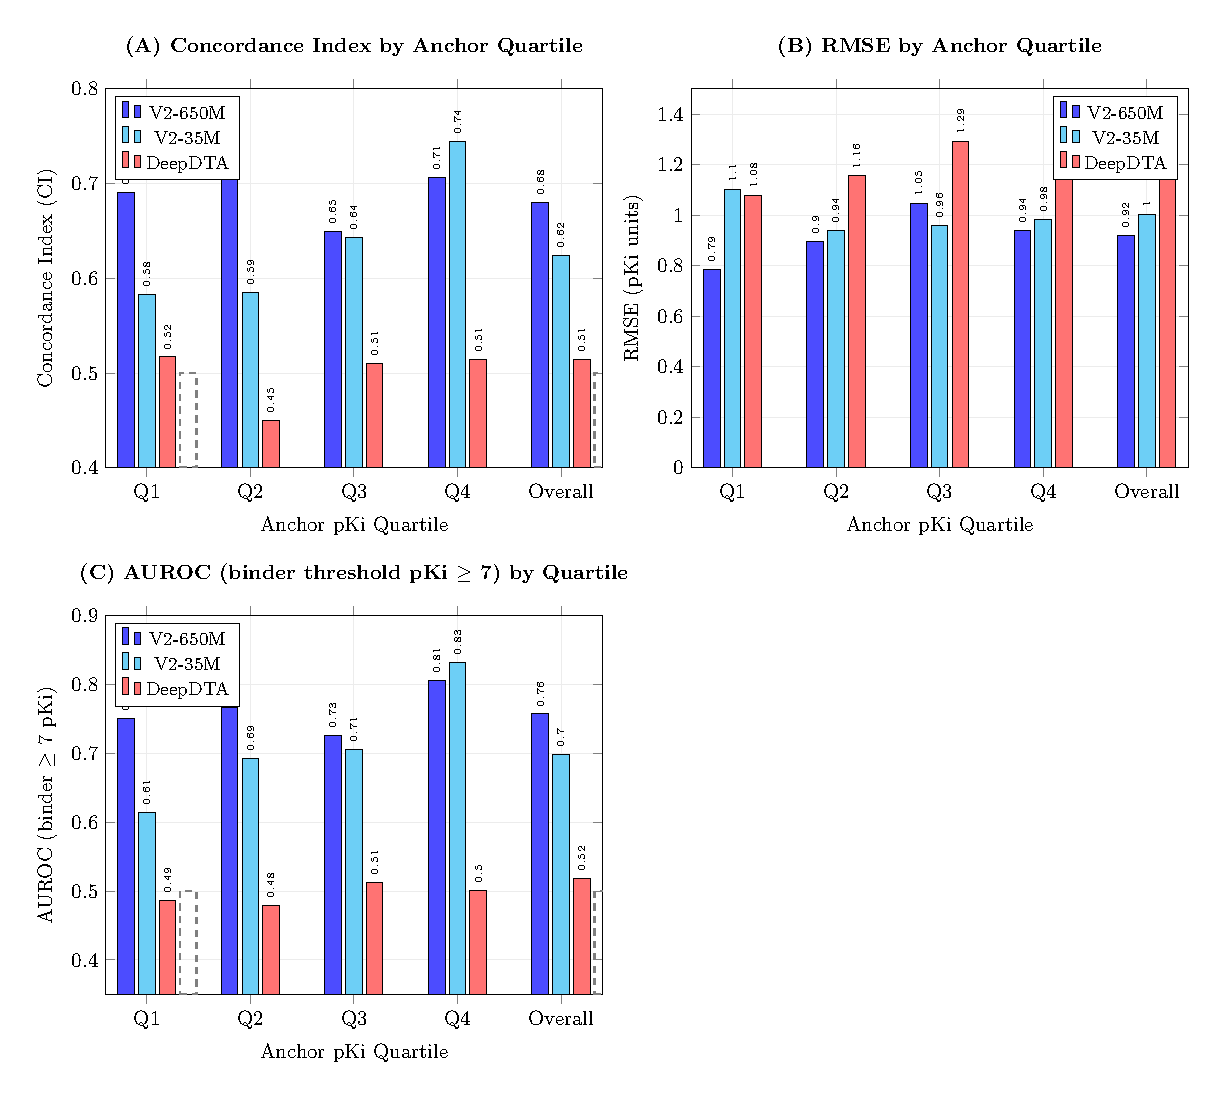
\includegraphics[width=\textwidth]{fig_davis_quartile_performance.pdf}
    \caption{Davis performance by oracle anchor quartile. \textbf{(A)}~Concordance index: V2-650M dominates in Q1--Q2 (weak anchors), while V2-35M overtakes in Q4 (strong anchors). DeepDTA is near-random throughout. \textbf{(B)}~RMSE: V2-650M achieves the lowest error in Q1 (0.786) where the anchor signal is weakest. \textbf{(C)}~AUROC with binding threshold pKi~$\geq$~7: both V2 variants substantially outperform DeepDTA, which fails to exceed random (0.5) in any quartile.}
    \label{fig:davis_quartile_performance}
\end{figure}

\paragraph{Per-protein metric distributions.}
To examine whether the global improvements reflect consistent per-protein gains or are driven by a few outlier proteins, Figure~\ref{fig:davis_per_protein} shows violin plots of per-protein CI, RMSE, and AUROC across all 442 Davis kinases.
Table~\ref{tab:davis_per_protein} reports summary statistics.

\begin{table}[t]
    \centering
    \caption{Per-protein metric summary across 442 Davis kinases (oracle anchors). Each protein is evaluated independently over its 66-drug panel. V2-650M achieves the highest mean CI and AUROC; V2-ProstT5 achieves the lowest mean RMSE.}
    \label{tab:davis_per_protein}
    \begin{tabular}{lcccccc}
        \toprule
        & \multicolumn{2}{c}{CI $\uparrow$} & \multicolumn{2}{c}{RMSE $\downarrow$} & \multicolumn{2}{c}{AUROC $\uparrow$} \\
        \cmidrule(lr){2-3} \cmidrule(lr){4-5} \cmidrule(lr){6-7}
        Model & Mean & Median & Mean & Median & Mean & Median \\
        \midrule
        V2-650M  & \textbf{0.645} & \textbf{0.651} & 0.888 & 0.853 & \textbf{0.691} & \textbf{0.706} \\
        V2-35M   & 0.604 & 0.594 & 0.985 & 0.963 & 0.663 & 0.665 \\
        V2-ProstT5 & 0.610 & 0.603 & \textbf{0.831} & \textbf{0.809} & 0.635 & 0.639 \\
        ConPlex  & 0.567 & 0.581 & 5.720 & 5.701 & 0.535 & 0.556 \\
        ESM-DTA  & 0.496 & 0.496 & 1.311 & 1.274 & 0.499 & 0.485 \\
        DeepDTA  & 0.507 & 0.513 & 1.174 & 1.160 & 0.487 & 0.496 \\
        \bottomrule
    \end{tabular}
\end{table}

\begin{figure}[t]
    \centering
    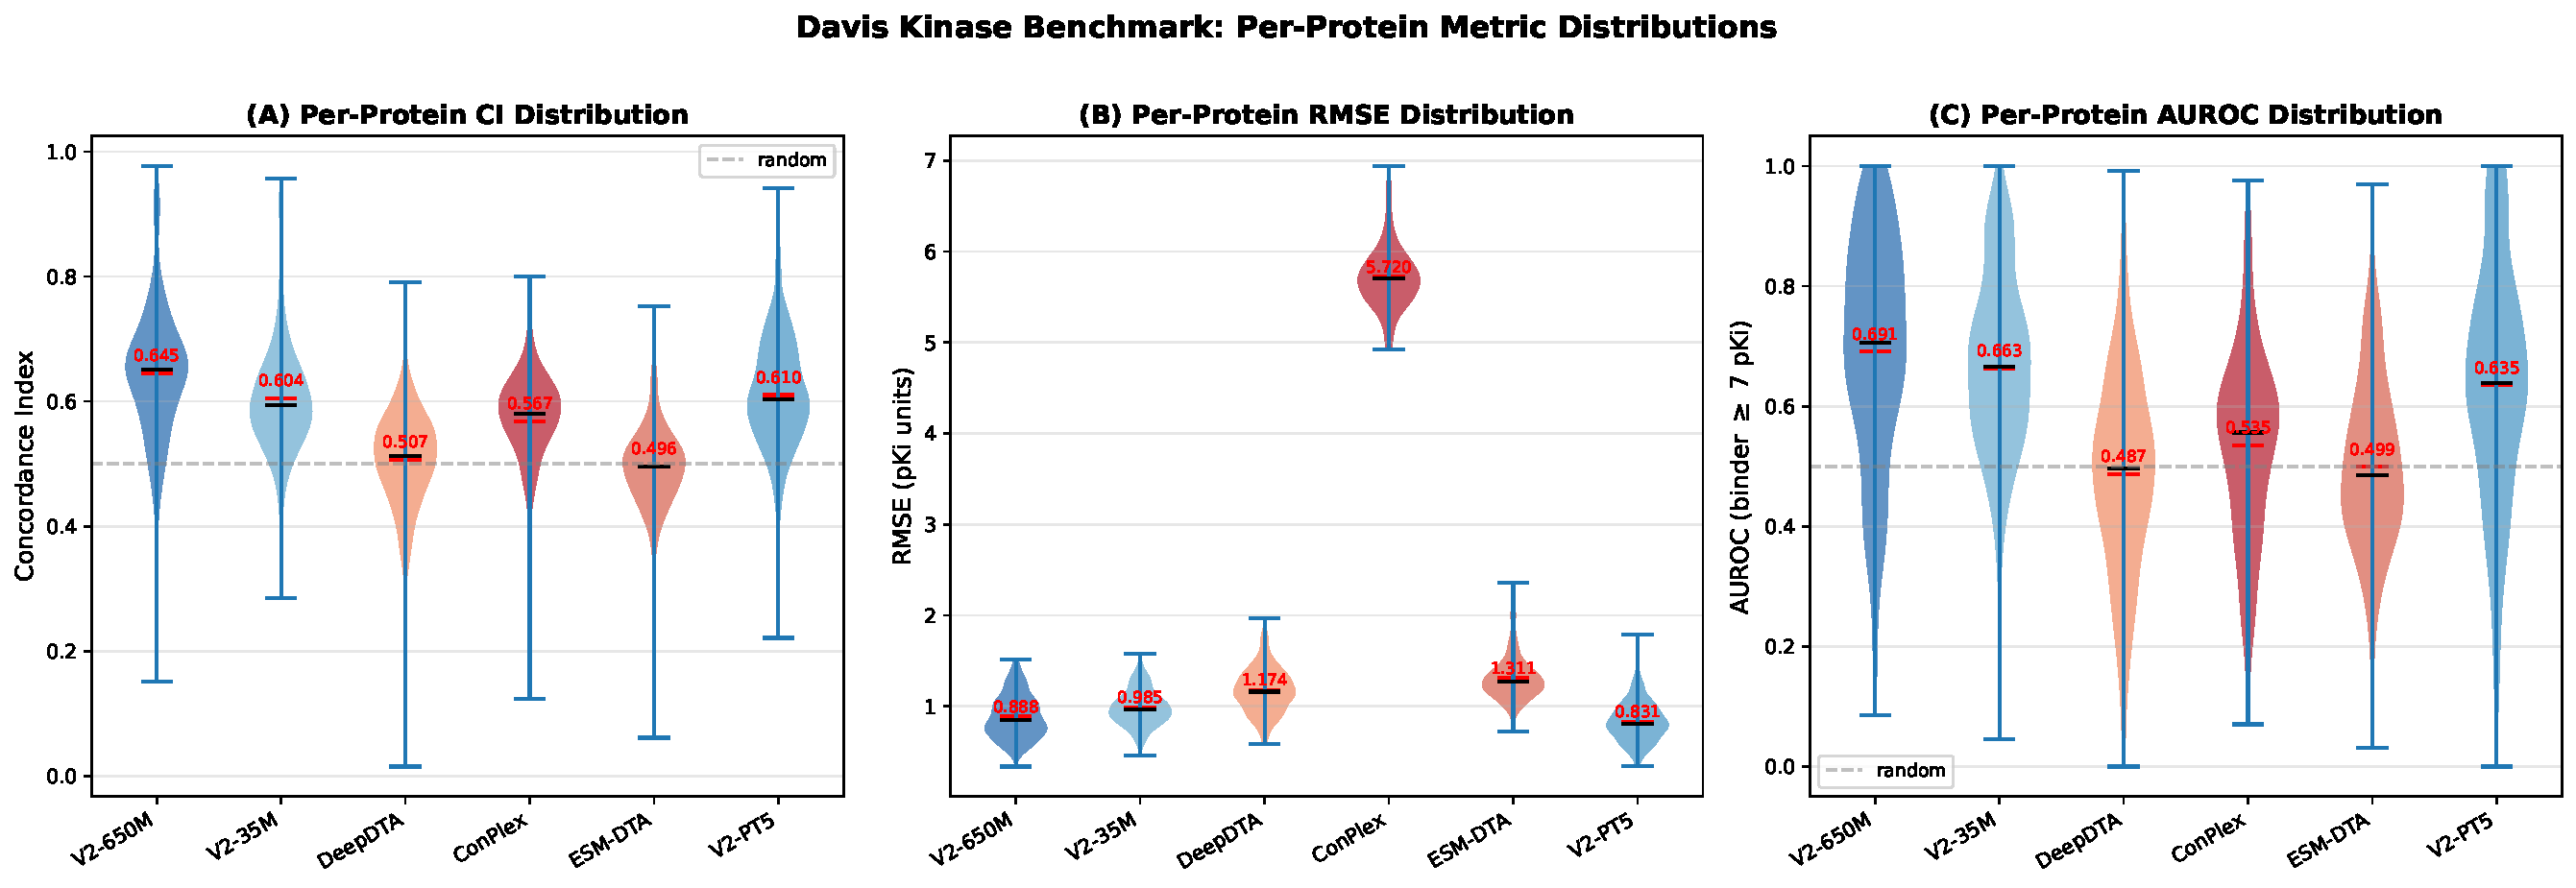
\includegraphics[width=\textwidth]{fig_davis_per_protein_distributions.pdf}
    \caption{Per-protein metric distributions on the Davis benchmark (442 kinases). Violin plots show the full distribution; red lines indicate means, black lines medians. \textbf{(A)}~CI: V2-650M has the highest median (0.651) and tightest distribution. DeepDTA and ESM-DTA cluster at random (0.5). \textbf{(B)}~RMSE: ConPlex has an extreme scale mismatch (mean 5.72); V2-ProstT5 achieves the lowest RMSE (0.831). \textbf{(C)}~AUROC (binder~$\geq$~7~pKi): V2-650M's distribution is shifted rightward; pairwise baselines center at random.}
    \label{fig:davis_per_protein}
\end{figure}

\paragraph{Interpretation.}
Three findings emerge from the anchor-stratified analysis:

\textit{1.~Pairwise models fail entirely on out-of-distribution kinases.}
DeepDTA achieves per-protein CI~$= 0.507$ and AUROC~$= 0.487$---indistinguishable from random.
ESM-DTA performs similarly (CI~$= 0.496$, AUROC~$= 0.499$).
Both models encode the target protein's sequence directly, and because the Davis kinases are absent from the DTC training set, the sequence encoder has no mechanism to transfer knowledge from related proteins.
ConPlex achieves slightly better CI (0.567) through its contrastive ESM-2 protein embedding, but its RMSE is catastrophic (5.72) because its scoring function is not calibrated to predict pKi values.
These results confirm that pairwise sequence-based models are fundamentally limited for cross-dataset generalization.

\textit{2.~The 650M encoder compensates for weak anchors.}
V2-650M's advantage over V2-35M is largest in Q1 and Q2 (weak anchors, pKi 7.0--9.1): CI 0.691 vs.\ 0.583 in Q1, and 0.706 vs.\ 0.585 in Q2.
When the anchor provides only a weak binding signal, the larger protein encoder extracts more discriminative information from the protein representation to compensate.
In Q1, V2-650M also achieves the lowest RMSE of any quartile (0.786), demonstrating accurate value prediction even with weak anchor reference points.

\textit{3.~Strong anchors equalize encoder capacity.}
In Q4 (strong anchors, pKi 9.6--10.8), V2-35M overtakes V2-650M (CI 0.744 vs.\ 0.706, AUROC 0.832 vs.\ 0.806).
When the anchor provides a high-affinity reference point, even a smaller encoder can exploit the relative binding signal effectively---the anchor's strong binding to the drug constrains the prediction space sufficiently that additional encoder capacity yields diminishing returns.
This suggests that anchor quality and encoder capacity are partially substitutable: a strong anchor compensates for a weaker encoder, and a strong encoder compensates for a weaker anchor.

\textit{4.~ProstT5 structure-aware embeddings improve calibration but not ranking.}
V2-ProstT5 achieves the lowest per-protein RMSE (0.831, lower than V2-650M's 0.888) but lower CI (0.610 vs.\ 0.645).
ProstT5's structure-aware embeddings produce better-calibrated absolute pKi predictions, while ESM-2 650M's sequence embeddings produce better relative rankings.
This trade-off suggests that combining both embedding types could improve both calibration and discrimination.

\subsection{Ablation: Cosine Similarity vs.\ Learned Representations}
\label{sec:cosine_ablation}

A natural question is whether anchor transfer simply exploits protein similarity---predicting that proteins similar to a known binder will also bind---or whether the model learns drug-specific binding patterns beyond raw similarity. To answer this, we compare the V2-650M model's predictions against a simple baseline: the cosine similarity between the anchor and query protein embeddings, used directly as a predictor of binding affinity.

Table~\ref{tab:cosine_ablation} reports per-protein AUROC and CI for cosine similarity predictors using three embedding spaces, compared against the full V2-650M model.

\begin{table}[t]
    \centering
    \caption{Cosine similarity between anchor and query protein embeddings as a standalone binding predictor on Davis, compared to the full V2-650M model. Per-protein metrics averaged over 442 kinases. Cosine similarity captures some binding signal but substantially underperforms the learned model, which additionally encodes drug structure and three-way interactions.}
    \label{tab:cosine_ablation}
    \begin{tabular}{lcccc}
        \toprule
        Predictor & AUROC $\uparrow$ & CI $\uparrow$ & Spearman $\rho$ & Binder--non-binder $\Delta\cos$ \\
        \midrule
        \textbf{V2-650M (full model)} & \textbf{0.691} & \textbf{0.645} & --- & --- \\
        \midrule
        Cosine (ProstT5) & 0.658 & 0.582 & 0.146 & 0.068 \\
        Cosine (ESM-2 650M) & 0.574 & 0.552 & 0.141 & 0.028 \\
        Cosine (ESM-2 35M) & 0.545 & 0.539 & 0.083 & 0.015 \\
        \bottomrule
    \end{tabular}
\end{table}

\paragraph{Similarity is necessary but not sufficient.}
Cosine similarity between anchor and query embeddings does carry binding-relevant signal: proteins that bind the same drug tend to have more similar embeddings than non-binders ($\Delta\cos = 0.028$ for ESM-650M, $0.068$ for ProstT5). This signal is statistically significant (Spearman $\rho = 0.14$, $p < 10^{-100}$) and produces above-random per-protein AUROC (0.574 for ESM-650M, 0.658 for ProstT5). However, cosine similarity alone is far weaker than the full model: V2-650M achieves AUROC 0.691 and CI 0.645, representing a 20\% relative improvement over the best cosine baseline (ProstT5, AUROC 0.658).

\paragraph{The model learns more than similarity.}
The V2-650M model's predictions correlate only weakly with the cosine similarity of its own embedding space (Spearman $\rho = 0.257$ between V2 predictions and ESM-650M cosine). This means 74\% of the model's predictive variance is orthogonal to raw protein similarity. The three pairwise interaction modules---anchor--drug, query--drug, and anchor--query---capture drug-specific binding patterns that pure protein similarity cannot encode. In a per-protein comparison, V2-650M outperforms ESM-650M cosine similarity on 361 of 442 proteins (82\%), ties on 20, and loses on only 61.

\paragraph{Structure-aware embeddings improve the similarity signal.}
ProstT5 embeddings, which encode 3Di structural alphabet features from Foldseek \cite{van2024fast}, produce the strongest cosine similarity baseline (AUROC 0.658, $\Delta\cos = 0.068$). This is consistent with ProstT5's superior performance in the anchor transfer framework (V2-ProstT5-BDB global AUROC 0.768): structure-aware embeddings better capture the structural similarity between anchor and query proteins that underlies binding knowledge transfer.

\paragraph{Implications.}
This ablation demonstrates that anchor transfer is not reducible to protein similarity matching. The model leverages similarity as one input signal but learns additional drug-specific and interaction-specific patterns through its three-way architecture. The anchor mechanism provides a structured comparison framework---``how does this query compare to a known binder for this specific drug?''---that goes beyond asking ``how similar are these two proteins?'' This distinction is important because it means the model can discriminate between drugs even when the anchor--query similarity is constant, by learning how different chemical scaffolds interact differently with the anchor--query protein pair.

\subsection{Ablation: Oracle Anchor Selection}
\label{sec:oracle_anchors}

The main cross-dataset results (Table~\ref{tab:davis_cross_dataset}) use realistic anchors retrieved by Tanimoto similarity after excluding canonical duplicates. As an ablation, we compare against oracle anchor selection, where the strongest known binder of each drug \emph{within the Davis evaluation set itself} serves as anchor---providing an upper bound that requires privileged access to evaluation data.

With oracle anchors (restricted to pKi~$\geq 7$, $n = 29{,}170$), V2-650M achieves per-protein CI 0.645 and AUROC 0.691. This is slightly higher than the realistic protocol (CI 0.642, AUROC 0.669), as expected since oracle anchors select the globally strongest binder rather than the nearest training-set analog. The gap is modest ($\Delta$CI $= 0.003$, $\Delta$AUROC $= 0.022$), confirming that Tanimoto retrieval produces anchors of comparable quality to oracle selection for this benchmark. Pairwise baselines remain near random under both conditions.


\section{Discussion}

The central result of this study is that anchor-based transfer improves generalization because it changes the prediction problem itself. Standard drug-target affinity models learn an absolute mapping from a protein--drug pair to a binding score, which is fragile under dataset shift because the model must infer compatibility from representations alone. Our anchor formulation instead asks a relative question: given that anchor protein $a$ is already known to bind drug $d$ strongly, how should query protein $q$ be scored relative to $a$ for the same drug? This is more transferable because it conditions prediction on experimentally grounded binding evidence rather than requiring the model to recover binding from sequence and chemistry alone. The anchor acts as a task-specific reference state, turning prediction from ``does $q$ bind $d$?'' into ``how does $q$ compare with a known binder of $d$?'' This reframing is consistent with findings in the transfer learning literature that relative or relational representations generalize better across domains than absolute features \cite{pan2010transfer,zhuang2021transfer}.

\subsection{What Anchor Transfer Actually Learns}

The anchor-stratified analysis on Davis (Section~\ref{sec:anchor_quartile}) provides direct evidence for what anchor transfer learns. Three observations are particularly revealing.

First, pairwise models (DeepDTA, ESM-DTA) achieve CI~$\approx 0.5$ on Davis---indistinguishable from random---despite strong performance on DTC (CI~$> 0.77$). These models have seen 77\% of Davis proteins during training (with different drugs), yet they cannot transfer binding knowledge to novel compounds even when evaluated with realistic Tanimoto-retrieved anchors. This confirms that pairwise architectures memorize protein--drug co-occurrences rather than learning transferable binding determinants.

Second, the complementary relationship between anchor quality and encoder capacity reveals the mechanism of transfer. V2-650M dominates in Q1--Q2 (weak anchors, pKi 7.0--9.1), achieving CI 0.691 versus 0.583 for V2-35M. But in Q4 (strong anchors, pKi 9.6--10.8), V2-35M overtakes V2-650M (CI 0.744 vs.\ 0.706). This trade-off has a natural interpretation: when the anchor provides a strong binding reference point, even a modest protein encoder can exploit the relative signal---the anchor constrains the prediction space sufficiently that additional encoder capacity yields diminishing returns. When the anchor is weak, the model must rely more heavily on the protein representation to discriminate, and the larger encoder compensates. Anchor quality and encoder capacity are partially substitutable resources for the same underlying task: estimating how a query protein's binding potential compares to that of a known binder.

Third, the per-protein metric distributions (Figure~\ref{fig:davis_per_protein}) confirm that V2-650M's advantage is consistent across proteins, not driven by outliers. The CI distribution is shifted rightward (mean 0.642) compared to baselines that cluster at random (DeepDTA 0.520, ESM-DTA 0.501). This consistency indicates that anchor transfer captures a general property of protein--drug binding rather than exploiting dataset-specific shortcuts.

\subsection{The Role of Protein Structural Similarity}

The success of anchor transfer rests on an implicit assumption: that structurally or functionally similar proteins bind similar drugs with predictable affinity relationships. The model does not receive explicit structural information---it operates on frozen protein language model embeddings---but the anchor mechanism creates an inductive pathway through which structural similarity becomes functionally relevant.

When the model is given an anchor protein that binds a drug strongly, it implicitly learns to compare the query protein's representation against the anchor's. If the two proteins share structural features relevant to binding (conserved active sites, similar fold topology, compatible binding pockets), the model can transfer the anchor's binding evidence to predict the query's affinity. The ESM-2 embeddings capture aspects of protein structure through their pre-training on evolutionary data \cite{lin2023esm2}, and the anchor mechanism leverages this structural signal in a binding-specific way.

This interpretation is supported by the ProstT5 results. V2-ProstT5-BDB achieves the highest global AUROC on Davis (0.768), surpassing V2-650M-DTC (0.757). ProstT5 \cite{heinzinger2023prostt5} is explicitly trained on 3Di structural alphabet representations from Foldseek \cite{van2024fast}, making its embeddings directly structure-aware. The fact that structure-aware embeddings improve anchor transfer performance suggests that the model benefits from better encoding of the structural similarity between anchor and query proteins.

The practical implication is that anchor transfer is most effective when the training set contains proteins that are structurally related to the evaluation targets. DTC-trained models benefit from 77\% protein sequence overlap with Davis, providing the model with anchor proteins from the same kinase family. BDB-trained models, which have broader protein diversity but less kinase enrichment, achieve lower Davis CI (0.602 for V2-35M-BDB vs.\ 0.624 for V2-35M-DTC). However, anchor quality filtering partially compensates: removing anchors with pKi~$< 7$ improves V2-650M-BDB global AUROC from 0.615 to 0.698, demonstrating that anchor quality matters more than anchor quantity.

\subsection{Limitations and the Need for Deeper Models}

Despite the strong results on Davis, several limitations indicate that deeper models and more diverse training data are needed for truly general-purpose drug-target affinity prediction.

\paragraph{Scope of generalization: compound novelty, not protein family novelty.}
We emphasize that our claim is \emph{not} that anchor transfer generalizes to protein families the model has never seen. The DTC training set shares 77\% of its proteins with Davis by sequence, and BDB shares 84\%. What the model has learned is a \emph{general representation of how drugs interact with known protein families}: given a protein that is structurally related to proteins in the training set, and given a known strong binder of a chemically similar drug, the model can predict whether the query protein will bind a novel compound. This is compound novelty---new drugs for known protein families---which is the dominant scenario in practical drug discovery (lead optimization, scaffold hopping, selectivity profiling, repurposing \cite{pushpakom2019drug_repurposing}).

For the model to generalize to entirely novel protein families, it would need training data spanning a broader range of protein structures and binding modes. The contrast between DTC-trained and BDB-trained models illustrates this directly: BDB has greater protein diversity but less kinase enrichment, and its models achieve lower Davis CI (0.602 vs.\ 0.624 for V2-35M). Broader generalization requires more proteins and more drugs---anchor transfer provides the mechanism, but the mechanism's reach is bounded by the structural diversity of the training data.

\paragraph{Drug overlap is deeper than SMILES strings suggest.}
A critical finding of our overlap audit (Table~\ref{tab:overlap_audit}) is that raw SMILES string comparison dramatically underestimates true drug overlap: while 0\% of Davis drugs match DTC by string identity, 83.8\% match by canonical SMILES and 89.7\% by InChIKey. Most Davis kinase inhibitors are literally present in DTC under different string representations. We address this by explicitly excluding all canonical duplicates from the anchor retrieval pool before evaluation, ensuring genuine zero molecular overlap.

After exclusion, the Tanimoto similarity distribution between Davis drugs and their nearest DTC match spans a wide range (12 drugs below 0.4, 22 between 0.4--0.6, 18 between 0.6--0.8). Table~\ref{tab:tanimoto_strat} shows that anchor transfer works even for chemically dissimilar compounds: the [0--0.6) bin (34 drugs with no close DTC analog) achieves CI 0.656 and AUROC 0.651. The best performance occurs at moderate similarity [0.6--0.8) (CI 0.708, AUROC 0.778), where the anchor's drug is structurally related but not identical to the query drug---providing useful binding context without redundancy.

This analysis has broader implications for the DTA literature. Many cross-dataset evaluations report zero drug overlap based on string comparison alone, which we show can mask near-complete molecular overlap. We recommend that future DTA benchmarks verify overlap at the canonical SMILES or InChIKey level to ensure genuine compound novelty.

\paragraph{Shallow architecture limits expressivity.}
The current architecture uses three independent pairwise MLPs (anchor--drug, query--drug, anchor--query) without higher-order interactions. This design is intentionally simple to isolate the contribution of the anchor mechanism from architectural complexity. However, it limits the model's ability to capture complex three-way relationships. Attention-based fusion, graph neural networks over the anchor--query--drug triplet, or deeper cross-attention modules could improve the model's capacity to reason about structural compatibility. The anchor quality--encoder capacity trade-off (Section~\ref{sec:anchor_quartile}) suggests that deeper models would most benefit the weak-anchor regime, where the current architecture already shows the largest gains from scaling ESM-2.

\paragraph{Training data diversity.}
The contrast between DTC-trained and BDB-trained models highlights the importance of training data composition. DTC is kinase-enriched, which helps on the kinase-focused Davis benchmark. BDB is broader but noisier, with 36\% of anchors having pKi~$< 7$ (weak or non-binding). Training on curated, structurally diverse datasets with verified high-quality binding data---such as filtered BindingDB with anchor quality thresholds---is likely to improve generalization to non-kinase families. The improvement from anchor quality filtering (pKi~$\geq 7$) already demonstrates this principle.

\paragraph{Anchor retrieval and future directions.}
The main evaluation uses Tanimoto chemical similarity for anchor retrieval, which requires no privileged access to evaluation data. More sophisticated retrieval strategies---learned retrieval modules that estimate transfer utility, or multi-anchor ensembles that aggregate evidence from several known binders---could further improve performance and provide calibrated uncertainty when anchors disagree. These extensions would be especially valuable for compounds with low Tanimoto similarity to the training set, where the current nearest-neighbor retrieval is weakest.

\subsection{Broader Implications}

These results suggest that cross-dataset DTA should be approached as a \emph{knowledge transfer problem over known interactions}, not solely as a representation learning problem. The failure of ESM-DTA (the strongest same-dataset model, AUROC 0.707 on DTC test) to generalize (CI 0.501 on Davis) demonstrates that better protein representations alone do not solve the transfer problem. The anchor mechanism provides the missing ingredient: a way to condition predictions on experimentally grounded binding evidence, making the model's reasoning explicitly relational rather than implicitly associative.

Critically, the model learns how drug--protein--protein relationships work within known protein families. When the model encounters a query protein that is structurally similar to proteins in its training set, and the query drug has a chemical analog with known binding data, the anchor mechanism enables transfer of that binding knowledge. This is not a limitation but a precise characterization of the method's scope: anchor transfer works because it exploits the structural regularity of protein families to predict binding of novel compounds. Extending this to novel protein families requires broader training data---more proteins from diverse structural classes, paired with more drugs from diverse chemical series. The anchor transfer mechanism itself is family-agnostic; it is the training data that determines which families the model can serve.


\section{Conclusion}

We introduced Anchor Transfer Learning for drug--target affinity prediction, a framework that conditions each prediction on an anchor protein already known to bind the same drug. Rather than scoring protein--drug pairs in isolation, the method turns affinity prediction into a comparison against experimentally grounded binding evidence. The formulation requires no structural information and applies to any target for which binder annotations exist.

The central empirical finding is a generalization gap: models that rank highest within a single benchmark are not the models that transfer best. DeepDTA and ESM-DTA collapse to random performance on Davis kinases (per-protein CI 0.520 and 0.501 respectively), despite achieving strong same-dataset metrics on DTC. Anchor transfer reverses this pattern: V2-650M achieves per-protein CI of 0.642 and AUROC of 0.669 on Davis. Crucially, anchors are retrieved at test time from the training set by Tanimoto chemical similarity after excluding all canonical chemical duplicates (83.8\% of Davis drugs were present in DTC under different SMILES strings), ensuring genuine zero molecular overlap. Performance stratification by retrieval similarity confirms that the model generalizes even to chemically dissimilar compounds (Tanimoto~$< 0.6$: CI 0.656).

A cosine similarity ablation confirms that the model learns more than protein similarity: 74\% of V2-650M's predictive variance is orthogonal to embedding cosine distance, and the full model outperforms cosine similarity on 82\% of Davis proteins. The three-way interaction architecture captures drug-specific binding patterns that raw protein similarity cannot encode.

ESM-DTA serves as a critical negative control: it is the strongest same-dataset model (AUROC 0.910 on DTC) yet collapses to random on Davis (per-protein AUROC 0.503). This demonstrates that stronger protein embeddings alone do not solve the cross-dataset transfer problem---the anchor mechanism provides the missing ingredient by conditioning predictions on experimentally grounded binding evidence.

The method is designed for the common drug discovery setting where at least one strong binder of the query drug is already known---lead optimization, scaffold hopping, selectivity profiling, and repurposing all satisfy this condition. Several directions remain open: learned anchor retrieval to improve on the current Tanimoto nearest-neighbor strategy, multi-anchor ensembles for calibrated uncertainty, deeper cross-attention architectures for richer three-way interactions, and evaluation on structurally diverse protein families beyond kinases.


\bibliographystyle{unsrtnat}
\bibliography{references}

\end{document}
